\documentclass[11pt]{"article"}
\setlength{\parindent}{0pt}
\linespread{1.5}
\usepackage[margin=1in]{geometry}
\usepackage{graphicx}
\graphicspath{ {../Diagrams/} }
\usepackage{titlesec}
\newcommand{\sectionbreak}{\clearpage}
\usepackage{sidecap}
\usepackage[singlelinecheck=false, labelfont=bf]{caption}
\usepackage{verbatim}
\usepackage{setspace}
\pagenumbering{roman}

\begin{document}


\begin{titlepage}
\centering
{\huge Computational Modelling of the Marker-Induction Mechanism of Retinotopic Map Development\\}
\vspace{1cm}
{\Large Tom Bland\\}
\vspace{2cm}
Supervisor:\\
Dr. Stephen Eglen\\
\vspace{2cm}
Word count:\\
5929 words
\end{titlepage}


\newpage
\thispagestyle{empty}
\mbox{}

\pagebreak

\setcounter{page}{1}

\begin{Large}
\textbf{Summary}\\
\end{Large}

The connections between the retina and the brain display topographic patterns, whereby adjacent cells in the retina connect to adjacent regions of target structures. These connection patterns, known as retinotopic maps, are essential for the visual system to function correctly. Computational testing of theoretical models can be valuable in helping us to understand how these maps may be set up. Progress in the field, however, is limited by both a lack of availability of computer code for models, and a lack of understanding of the modelling process amongst experimental biologists. \\

In this project I aim to contribute to fixing this problem by recreating an influential theoretical model of retinotopic map formation: the marker-induction model. I provide a comprehensive account of the modelling process, which will be published in the form of a tutorial paper, and share the computer code for map formation online. I also address a number of limitations of the original model and overcome these with an updated form of the model. I show that my new model can account for a number of experimental observations, covering the effects of surgery and genetic manipulations on map formation, and use it to make novel predictions about the system. Analysis of maps produced by the model was performed using three newly developed map precision measures.


\tableofcontents

\section*{List of Abbreviations}

\begin{tabular}{ll}
PF & Projective Field \\
RF & Receptive Field \\
RGC & Retinal Ganglion Cell \\
SC & Superior Colliculus \\
TC & Tectal Cell \\
\end{tabular}


\section{Introduction}
\pagenumbering{arabic}

\textbf{Topographic maps}

Sensory pathways are responsible for converting physical or chemical stimuli into a complex pattern of electrical activity, giving us a perception of the world around us. All sensory pathways rely on structures in the peripheral nervous system to transduce stimuli into electrical activity, and structures in the central nervous system to process information. This setup requires long-range transfer of information between peripheral and central structures, which is facilitated by neural connections between sensory cells and central neurons.  
\\

Many sensory systems rely on spatial information to function. In the visual system, a spatial representation of the world is only possible if the retinal location of active photoreceptors is taken into account. In the auditory system, hair cell location along the cochlea determines their characteristic frequency of activation, so spatial information is required to allow us to discriminate pitch (Bekesy and Wever, 1960). It is therefore essential in these systems that spatial information in the periphery is accurately communicated to the central nervous system. In order to achieve this, sensory systems have developed orderly patterns of connections, known as topographic maps, which retain spatial information by connecting adjacent cells in sensory structures to adjacent cells in the target structures (figure 1).
\\

The mechanisms underlying the development of topographic maps have been the subject of research for many decades, but are still unclear (Bednar and Wilson, 2016). Detailed study of the development of specific maps can help us to understand the common mechanisms that underlie map formation across systems and across species. As well as sensory systems, topographic maps are found in systems such as the spinal cord, the hippocampus, and the motor system (O'Donovan, 1999). Understanding mechanisms of map development may be of clinical importance in helping us to understand how the nervous system might recover in response to injury.
\\

\pagebreak

\begin{SCfigure}[][!h]
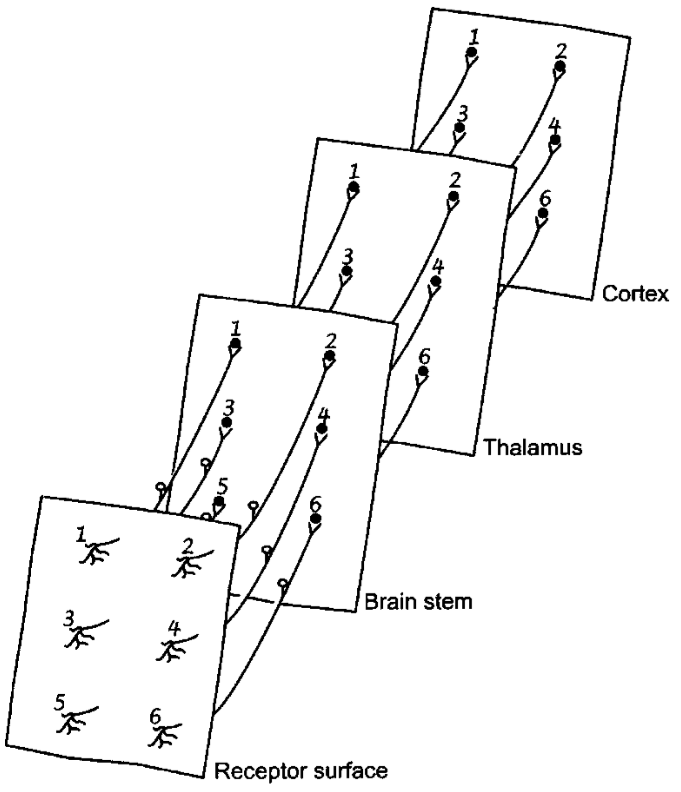
\includegraphics[scale=0.3]{Topography}
\caption{\setstretch{1.0}\textbf{Topographic maps in sensory systems.} 
Adjacent cells in the sensory receptor surface connect to adjacent regions of the target structure in the brainstem. Topography is retained in the connections between structures in later parts of the pathway. Figure from Kaas and Catania (2002).}
\end{SCfigure}

\vspace{15pt}

\textbf{Topography in the visual system}

The visual system contains a number of examples of topographic maps, which ensure that the spatial representation of the world that is projected onto the retina is not scrambled along the visual pathway. The best-studied example is the connections between retinal ganglion cells (RGCs) and cells of the tectum (known as the superior colliculus, SC, in mammals), a structure in the midbrain that carries out preliminary visual processing. This forms maps known as retinotopic maps.
\\

Development of retinotopic maps is traditionally thought to rely on two classes of mechanism: marker-dependent and activity-dependent (Eglen and Gjorgjieva, 2009). Marker-dependent mechanisms (described in detail in the following sections) are thought to act first, setting up global order in the map, and are followed by activity-dependent mechanisms, which act to enhance spatial continuity in maps and prune away excess connections (figure 2). This refinement is achieved through correlated activity in the retina and tectum, facilitated by short range excitatory, and long range inhibitory contacts within layers. Since synapses are modified according to their level of activity (Hebb, 1949), ordered activity favours ordered connections. 
\\

\pagebreak

\begin{SCfigure}[][!h]
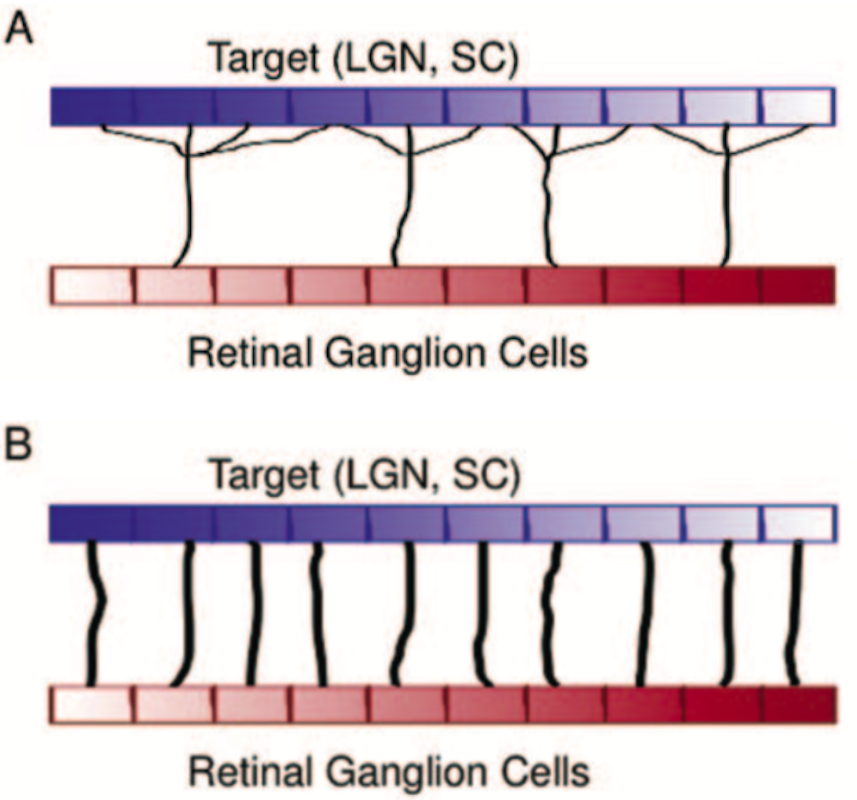
\includegraphics[scale=0.21]{TwoMechanisms}
\caption{\setstretch{1.0}\textbf{Two stages of retinotopic map development}
\textbf{(A)} Stage 1: Marker-dependent mechanisms set up topography, but RGCs connect to many target neurons with weak connections.
\textbf{(B)} Stage 2: Activity-dependent mechanisms refine maps, removing excess connections, and strengthening remaining connections.
Figure from Eglen and Gjorgjieva (2009)}
\end{SCfigure}

\vspace*{10pt}

\textbf{Molecular markers}

{\setstretch{1.4}
Marker-dependent mechanisms were first put forward by Sperry (1963), based on his experiments on amphibians. Importantly in adult amphibians and fish, retinotopic maps will reform after the optic nerve is cut and connections are allowed to re-establish. Sperry showed that if amphibian optic nerves are cut, and eyes rotated, then maps reform as usual, with RGCs connecting to the same tectal region as before. This suggests that RGCs have an innate preference for particular regions of the tectum. Sperry proposed that the retina and tectum contain gradients of molecular markers, allowing each cell to be labelled uniquely based on their set of marker concentrations. These markers distinguish individual cells within a sheet from one another, and allow RGCs to find their matching region in the tectum.  
\\

It was not until several decades later that molecules were identified with properties matching Sperry's hypothesis (Cheng et al., 1995). Map formation is now understood to rely on a system of Eph tyrosine-kinase receptor gradients in the retina, and ephrin ligand gradients in the tectum. Two Eph/ephrin systems (A and B) are used, which are set up as gradients along orthogonal axes in the structures (figure 3). The two systems differ in their receptor-ligand relationships: whereas RGCs with high EphA connect to TCs with low ephrinA, RGCs with high EphB connect to TCs with high ephrinB. Map formation is also aided by counter-gradients of ephrins in the retina and Ephs in the tectum. Overall these characteristic gradients and receptor-ligand relationships generate ordered maps with a well defined orientation (figure 3). The role of Ephs and ephrins in map formation has been confirmed by a number of studies genetically manipulating retinal and tectal Eph and ephrin gradients, which in many cases leads to abnormal maps (Brown et al., 2000; Feldheim et al., 2000; Reber et al., 2004).\par
}

\begin{SCfigure}[][!h]
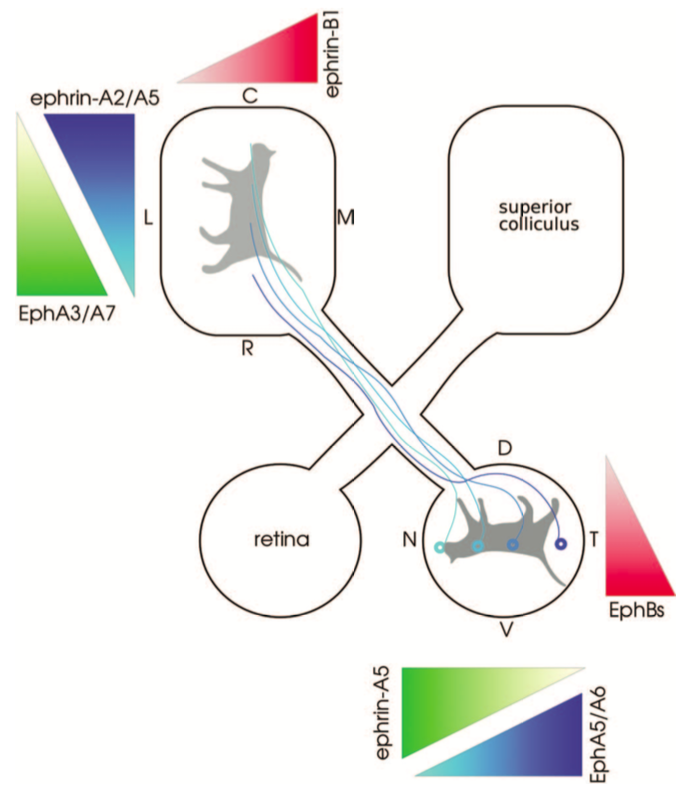
\includegraphics[scale=0.32]{Connections}
\caption{\setstretch{1.0}\textbf{Anatomy of retinotopic maps.} 
Each retina creates a topographic projection onto the contralateral SC (mammals) or tectum (non-mammals). The nasal (N) - temporal (T) axis of the retina projects onto the caudal (C) - rostral (R) axis of the tectum (referred to in this report as the posterior-anterior axis). The dorsal (D) - ventral (V) axis of the retina projects onto the lateral (L) - medial (M) axis of the tectum. This arrangement is brought about by orthogonal gradients of Eph (retina) and ephrin (tectum), and aided by counter-gradients. Figure from Eglen and Gjorgjieva (2009).}
\end{SCfigure}

\vspace*{25pt}

\textbf{Map plasticity}

Despite the identification of molecules that fit Sperry's hypothesis, it is far from being a complete picture of reality, and its simple nature leaves it unable to explain many observations. A particularly important observation is that, under certain experimental conditions, RGCs can be made to connect to tectal regions that they would not usually connect to in a normal adult map. This has been demonstrated by a number of mismatch experiments, which involve removing part of the retina and/or tectum after cutting the optic nerve, then allowing the connections to re-establish. These experiments show that systems-matching occurs, whereby maps adjust their connectivity to compensate for size differences between the layers (Gaze and Sharma, 1970; Horder, 1971; Schmidt et al., 1978). This contradicts Sperry's hypothesis, which proposes a strict matching between specific retinal and tectal regions.
\\

\pagebreak

\textbf{The marker-induction model}

{\setstretch{1.4}
Computer modelling has experienced rapid growth in neuroscience over the past several decades (Abbott, 2008), and has proved a valuable tool for a number of reasons. Firstly, the process of building formal computational models as a set of equations, rather than a set of words, can help to clarify ideas, and forces models to be complete and non-contradictory. Once built, computer models can then be used to test the feasibility of hypotheses, which is often easier, quicker and cheaper than testing them experimentally. Computational modelling can therefore save resources by acting as a useful initial filter of ideas before full experimental testing. 
\\

Research into topographic map development is no exception, and computational modelling has contributed greatly to our understanding of the problem (Goodhill, 2007). In the case of retinotopic maps, the earliest attempt to combine knowledge of molecular markers and map plasticity into a comprehensive model of map formation was the marker-induction model, initially proposed in 1977 (Malsburg and Willshaw, 1977) and fully described in 1979 (Willshaw and von der Malsburg, 1979), before the identification of Ephs and ephrins. This model attempts to explain map plasticity by proposing that tectal marker gradients are flexible, and can change to permit map changes. In the model, labelled RGCs initially connect randomly to the tectum, which contains no (or weak) gradients of label. RGCs continuously induce label into the TCs that they synapse on, the rate of which depends on the weight of the synapse, and markers are also transferred between adjacent cells in the tectal layer. Synaptic weights are updated continuously according to the complementarity in marker composition between the RGC and TC, meaning that synapses will be preferentially strengthened between cells with complementary labels, which is enhanced when adjacent TCs carry similar labels. This mechanism ensures that neighbouring cells connect to neighbouring cells, generating topography on a microscopic level. Size and location properties of the map are set by the boundaries of the layers, with maps automatically filling the two layers. A small initial bias, either in the pattern of initial connections or the initial tectal gradients, is required to give global order to the map, and to specify its orientation.
\\

Comprehensive computational analysis of the model on small one-dimensional collections of cells, using a set of arbitrary markers, demonstrated a good ability to predict systems-matching in mismatch surgery operations (Willshaw and von der Malsburg, 1979). The model was updated upon the discovery of the Eph/ephrin system (Willshaw, 2006), replacing arbitrary markers with gradients of Ephs and ephrins, and has demonstrated good ability to predict the effects of a number of genetic manipulations (Willshaw, 2006; Hjorth et al., 2015).
\par
}

\pagebreak

\textbf{Project aims}\\
As new experimental evidence becomes available, the marker-induction model must be continually tested and updated to stay relevant. Computer code of the model, however, is not readily available, and therefore further testing of its power requires researchers to rebuild the model from scratch, which is far from trivial. A major aim of this project was to aid this process by rebuilding the model in an accessible format, documenting the modelling process in the style of a tutorial paper, and sharing the computer code.\\

In rebuilding the model I also aimed to make a number of changes to it, by combining components of the original 1979 model and the updated 2006 model, in order to improve its power and biological relevance. I further aimed to build a full analysis toolkit to characterise, quantify and compare the success and progression of map formation between simulations. I demonstrate the power of my model and analysis toolkit by performing a range of simulations covering normal map development, the effects of surgery, and the effects of genetic manipulations. I also use it to make predictions about the necessary strength of initial tectal ephrin gradients.


\section{Methods}

\subsection{Model}

\vspace{10pt}

\textbf{Model overview}\\
The model used in this project combines the most biologically realistic features of the 2006 model and the 1979 model, to form a new \textit{hybrid} model. The 2006 model is clearly advantageous in its consideration of Eph and ephrin gradients, but lacks a consideration of the mechanisms of synaptic formation and removal, instead modelling every RGC as being at all times connected to every TC. This feature, however, is accounted for in the 1979 model, which includes reactions for synapse elimination below a threshold weight, and sprouting of new synapses from existing ones. My new model uses Eph and ephrin gradients, but incorporates the synapse formation and removal reactions from the 1979 paper. The reasons for including these reactions are twofold. Firstly, it makes the model more biologically realistic. Secondly, it allows some of the calculations to be limited to the small subset of RGC to TC interactions that actually have a synapse present, rather than all possible interactions, which greatly improves the computational performance of the model, and allows larger systems to be simulated. A more detailed account of the origin of each component of the new model can be found in table 1.\\ 

In building the model I began by rebuilding each original model from scratch using the information available in the original papers, expanding the 1979 model to two dimensions. Whilst the original papers contain all the equations and parameters required, information about modelling approaches is lacking, and therefore a large amount of work went towards developing a modelling approach. Once the original models were rebuilt, components of each model were combined to make the new model. It was necessary to alter a number of model parameters in light of these changes to improve model performance. Due to the large number of parameters and long running time of the model, a formal and complete parameter-optimisation algorithm was not viable. Instead, parameters were kept at their original value where possible, and a small number of alternative parameter sets was tested. Parameters were optimised to generate precise maps in normal development simulations (see section 3.1). A summary of parameters used in the model ($\alpha, \beta, \kappa, \gamma, K, W$ and $\Delta t $) is found in table 3.\\

\pagebreak

The key components of the model are layers of RGCs and TCs, which were modelled as two-dimensional rectangular grids of cells, where dimensions represent the two orthogonal anatomical axes for each structure. Cells were numbered according to their coordinates in their grid in the form $(i,j)$ for RGCs, where $i$ represents position along the nasal-temporal axis and $j$ represents position along the dorsal-ventral axis, and $(m,n)$ for TCs, where $m$ represents position along the posterior-anterior axis and $n$ represents position along the lateral-medial axis (figure 4).\\

\vspace*{20pt}

\begin{figure}[!h]
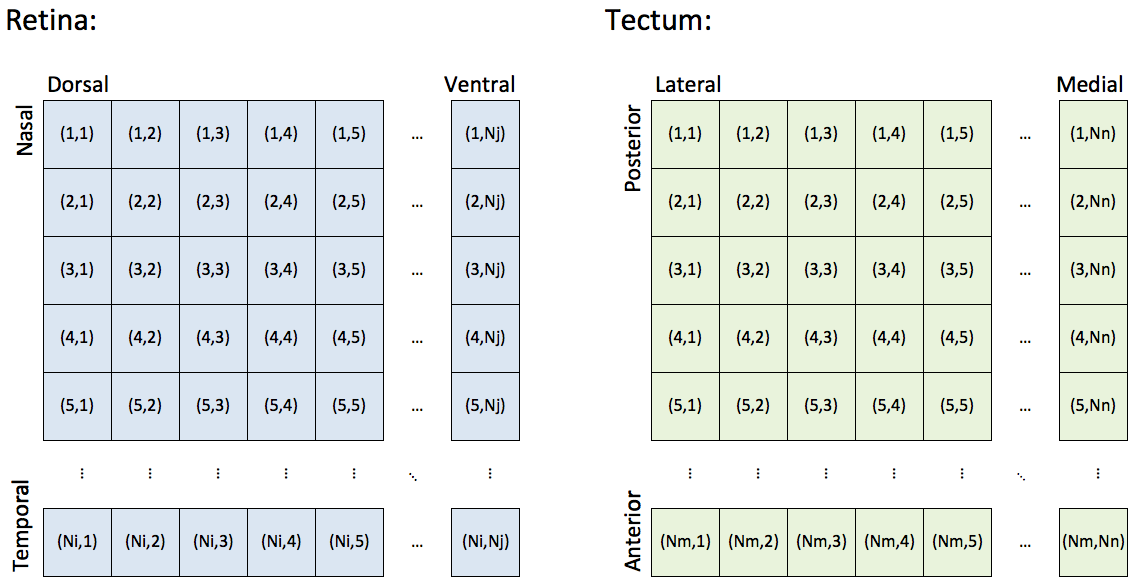
\includegraphics[scale=0.4]{Coordinates}
\setlength{\abovecaptionskip}{20pt}
\caption{\textbf{Retinal and tectal cell layers.}
Blue squares represent RGCs, green squares represent TCs. Each cell is given coordinates according to their position in their grid. Ni, Nj, Nm and Nn are the number of cells modelled in the nasal-temporal, dorsal-ventral, posterior-anterior and lateral-medial axes respectively.}
\end{figure}

\pagebreak

Each cell contains a set of Eph or ephrin markers of a certain density. RGCs contain a fixed density of EphA and EphB, $R_{(i,j)}^A$ and $R_{(i,j)}^B$ respectively. Likewise, TCs contain densities of ephrinA and ephrinB, $T_{(m,n)}^A$ and $T_{(m,n)}^B$ respectively, which are flexible throughout the simulation. Counter-gradients were not modelled. Axons connect each RGC to a subset of TCs, forming synapses of weight $W^{(i,j)}_{(m,n)}$, which depend on the complementarity in the marker sets ($\Phi^{(i,j)}_{(m,n)}$) between the RGC and the TC. A weight value of zero represents the lack of a synapse between a certain RGC and TC.\\

Simulations are initiated by setting up initial gradients and an initial random connectivity pattern. Simulations then follow an iterative process, where the following steps are carried out sequentially a number of times:\\
 
1) Tectal labels are updated by induction from RGCs and neighbouring TCs
 
2) Synaptic weights are modified according to the complementarity in the marker sets between the RGC and TC involved 

3) Synaptic weights are normalised to keep the total weight available to an RGC constant 

4) Synapses which have fallen below a threshold weight are removed

5) New synapses are formed by sprouting from existing synapses
\\

In the remainder of this section I describe the modelling approach I took for each of these processes in detail.\\


\pagebreak

\textbf{Initial gradients}\\
EphA and EphB densities are given as two orthogonal gradients across the retina, and the tectum is given initial weak orthogonal gradients of ephrinA and ephrinB. Gradients match those used by Willshaw (2006). EphA gradients are based on quantitative measurements (Reber et al., 2004), whereas EphB and ephrin gradients had to be estimated due to a lack of available data. Initial ephrin gradients follow the directions required to set up the correct map orientation, but must be overwritten and smoothened in the model to permit map topography. Default initial gradients are shown in figure 5.\\

\begin{figure}[!h]
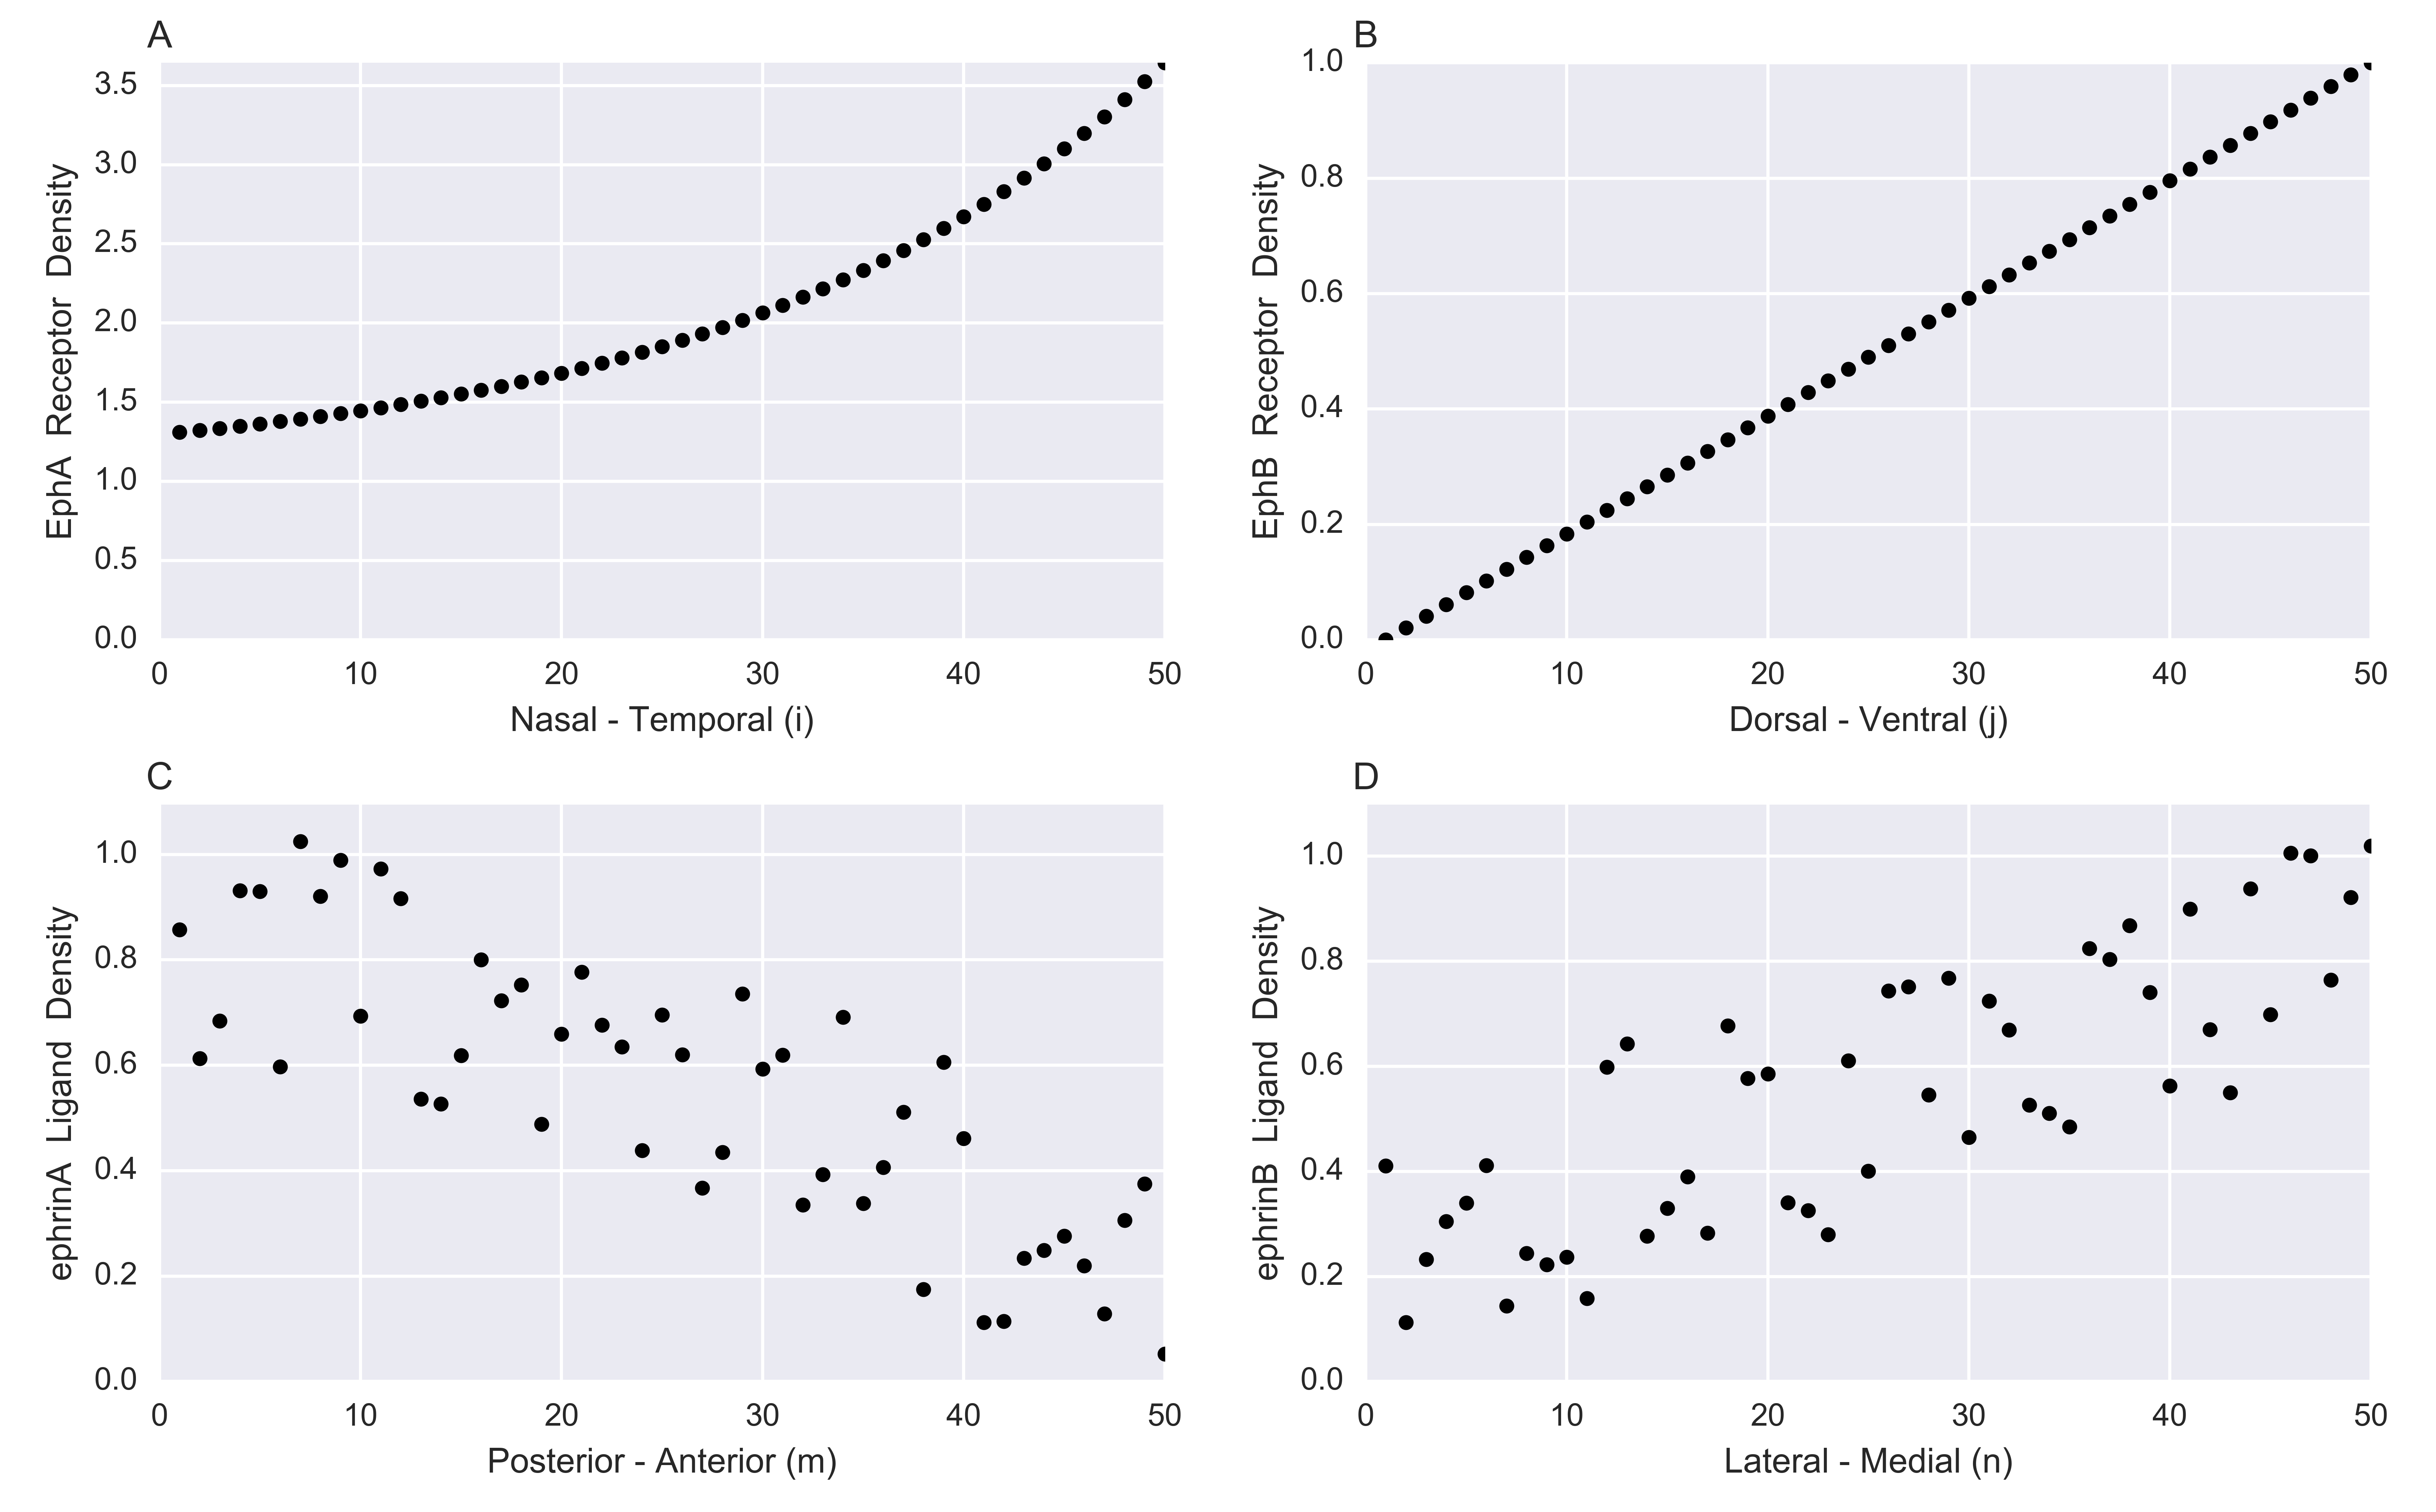
\includegraphics[scale=0.6]{Gradients}
\caption{\setstretch{1.0}\textbf{Initial Eph and ephrin gradients.} 
Data from a simulation with a 50x50 cell retina and a 50x50 cell tectum. Gradients are shown at a slice point half way along the length of the orthogonal axes. 
\textbf{(A)} EphA density across the nasal-temporal axis of the retina. Densities follow the equation $y = 0.26e^{2.3x} + 1.05$ (Reber et al., 2004), where $y$ is the density of label in a cell at a distance $x$ units along the axis (where $x$ is the nasal-temporal coordinate, i, normalised to 1)
\textbf{(B)} EphB density across the dorsal-ventral axis of the retina. \textbf{(C)} ephrinA density across the posterior-anterior axis of the tectum. Densities follow the equation $y = -0.6x + 0.5\Pi$, where $\Pi$ is a random number from 0 to 1 drawn for each individual cell. 
\textbf{(D)} ephrinB density across the lateral-medial axis of the tectum. Densities follow the equation $y = 0.6x + 0.5\Pi$}
\end{figure}

\pagebreak

\textbf{Label updating}\\
Tectal labels are produced or removed at a rate which depends on two factors: induced Eph in RGC axon terminals, and ephrin density in adjacent TCs. Induced Eph ($I_{(m,n)}^A$ and $I_{(m,n)}^B$ for EphA and EphB respectively) is defined as the total density of Eph in the RGCs innervating a TC, weighted by synapse strength:

\begin{equation}
I_{(m,n)}^A = \frac{\Sigma_{(i,j)} W^{(i,j)}_{(m,n)} R_{(i,j)}^A}{\Sigma_{(i,j)} W^{(i,j)}_{(m,n)}}
\end{equation} 

\begin{equation}
I_{(m,n)}^B = \frac{\Sigma_{(i,j)} W^{(i,j)}_{(m,n)} R_{(i,j)}^B}{\Sigma_{(i,j)} W^{(i,j)}_{(m,n)}}
\end{equation}\\

The influence of these values on ephrin production depends on the Eph/ephrin system. $T_{(m,n)}^B$ changes until it matches $I_{(m,n)}^B$, whereas $T_{(m,n)}^A$ changes until it matches $1 / I_{(m,n)}^A$ (equations 3 and 4, first term). This ensures that RGCs with high EphB connect to TCs with high ephrinB, and RGCs with high EphA connect to TCs with low ephrinA.  The second term in the equations represents communication between neighbours, which ensures spatial continuity in the tectum, and permits formation of even maps. Label production is regulated according to the difference between the density of a label in a cell and the mean density in its neighbours ($N_{(m,n)}^A$ and $N_{(m,n)}^B$ for ephrinA and ephrinB respectively). Note that this is a slight deviation from the 2006 model, where the Laplacian operator was used to calculate neighbour communication.

\begin{equation}
\Delta T_{(m,n)}^A = [\alpha (1 - I_{(m,n)}^A T_{(m,n)}^A) + \beta (N_{(m,n)}^A - T_{(m,n)}^A)] \Delta t
\end{equation}

\begin{equation}
\Delta T_{(m,n)}^B = [\alpha (I_{(m,n)}^B - T_{(m,n)}^B) + \beta (N_{(m,n)}^B - T_{(m,n)}^B)] \Delta t
\end{equation}

\textit{where}

\begin{equation}
N_{(m,n)}^A = \frac{T_{(m+1,n)}^A + T_{(m-1,n)}^A + T_{(m,n+1)}^A + T_{(m,n-1)}^A}{4}
\end{equation}

\begin{equation}
N_{(m,n)}^B = \frac{T_{(m+1,n)}^B + T_{(m-1,n)}^B + T_{(m,n+1)}^B + T_{(m,n-1)}^B}{4}
\end{equation}

\textbf{Boundary conditions}\\
Cells on the edge of a layer have fewer than 4 neighbours, so have to be treated differently. Particularly important is the neighbour communication term, which takes inputs from 4 adjacent cells. This poses a problem for cells on the edges, which have three neighbours, and on the corners, which have just two neighbours. To allow a single function to be used for all cells, matrices were written to contain a layer of \textit{zero padding} on the outside. For example, if 50 cells are being used for a dimension in a simulation, this effectively creates cells at coordinates 0 and 51 with marker densities fixed at zero. To ensure that label is not lost from the edge of layers (i.e. boundaries are reflective) the denominator in equations 5 and 6 is set to represent the number of direct neighbours a cell has, so will be lower for edge (denominator $=$ 3) and corner (denominator $=$ 2) cells. 
\\

\textbf{Weight updating}\\
Each RGC initially makes 10 synapses of equal weight with random TCs. With each iteration, synaptic weights are updated according to the marker complementarity ($\Phi^{(i,j)}_{(m,n)}$) between the RGC and TC involved, which is calculated based on the distance measure $\Psi^{(i,j)}_{(m,n)}$:

\begin{equation}
\Psi^{(i,j)}_{(m,n)} = (R_{(i,j)}^A T_{(i,j)}^A - 1)^2 + (R_{(i,j)}^B - T_{(i,j)}^B)^2
\end{equation}

\begin{equation}
\Phi^{(i,j)}_{(m,n)} = exp\left[\frac{\Psi^{(i,j)}_{(m,n)}}{2\kappa ^2}\right]
\end{equation}

The synaptic weight change is then calculated according to the complementarity between the RGC and TC involved:

\begin{equation}
\Delta W^{(i,j)}_{(m,n)} = \left[ (\Phi^{(i,j)}_{(m,n)} - \phi^{(i,j)}) + K \right] \gamma \Delta t 
\end{equation}

where $\phi^{(i,j)}$ is the mean complementarity between an RGC and all the TCs that it is connected to. To calculate new synaptic weights ($\bar{W}$), weight changes are normalised to keep the total synaptic weight available to each RGC at a constant value, $w$:

\begin{equation}
\bar{W}^{(i,j)}_{(m,n)} = \frac{ [W^{(i,j)}_{(m,n)} + \Delta W^{(i,j)}_{(m,n)}] w}{w + \Sigma_{(m,n)} \Delta W^{(i,j)}_{(m,n)} }
\end{equation}
\\

\textbf{Sprouting and synapse removal}\\
With each weight update iteration, all synapses of weight below $0.5\%$ of $w$ are removed. Each synapse of weight greater than $2\%$ of $w$ then sprouts new synapses of weight $1\%$ of $w$ onto each adjacent TC that the axon doesn't already contact.
\\\\

\textbf{Summary of model components}\\

\begin{table}[h]
\setstretch{1.5}
\caption{\textbf{Origin of model features}}
\begin{tabular}{|l|l|l|}
\hline
Model Feature & Equation(s) & Origin \\
\hline
Eph/ephrin gradients & Fig 5 legend & Willshaw (2006) \\
Induced label & 1,2 & Willshaw (2006) \\
Neighbour communication & 5,6 & Adapted from Willshaw (2006) \\
Tectal label updating & 3,4 & Adapted from Willshaw (2006) \\
Marker complementarity & 7,8 & Willshaw (2006) \\
Weight change & 9 & Willshaw and von der Malsburg (1979) \\
Weight normalisation & 10 & Willshaw and von der Malsburg (1979) \\
Sprouting/synapse removal & - & Willshaw and von der Malsburg (1979) \\
\hline
\end{tabular}
\end{table}

\vspace*{15pt}

\begin{table}[h]
\setstretch{1.5}
\caption{\textbf{Model variables}}
\begin{tabular}{|c|l|}
\hline Variable & Biological Meaning \\ \hline
$R_{(i,j)}^{A/B}$ & RGC EphA/B density \\
$T_{(i,j)}^{A/B}$ & TC ephrinA/B density \\
$I_{(m,n)}^{A/B}$ & Induced EphA/B  \\
$N_{(m,n)}^{A/B}$ & Mean neighbour ephrinA/B density \\
$\Phi^{(i,j)}_{(m,n)}$ & Marker set distance \\
$\Psi^{(i,j)}_{(m,n)}$ & Marker set complementarity \\
$W^{(i,j)}_{(m,n)}$ & Synaptic weight \\ \hline
\end{tabular}
\end{table}

\pagebreak
\begin{table}[h]
\setstretch{1.5}
\caption{\textbf{Model parameters}}
\begin{tabular}{|c|c|c|c|l|}
\hline Parameter & 1979 & 2006 & Hybrid Model & Biological Meaning \\ \hline
$\alpha$ & - & 0.05 & 0.05 & Strength of marker induction  \\
$\beta$ & - & 0.01 & 0.05 & Strength of neighbour communication \\
$\kappa$ & - & 0.0504 & 0.5 & Sharpness of receptor-ligand comparison  \\
$\gamma$ & 0.01 & 0.1 & 0.1 & Rate of weight update \\
$K$ & 0.03 & - & 0.005 & Basal rate of synaptic strengthening \\
$W$ & 1 & 1 & 1 & Total weight available to an RGC \\
$\Delta t$ & 1 & 0.1 & 1 & Time step \\ \hline
\end{tabular}
\end{table}
\pagebreak

\subsection{Data Analysis}

\textbf{Characterising receptive fields}\\
Once simulations are run, the data produced, which takes the form of a synaptic weight matrix between all RGCs and TCs, must be analysed. To begin this analysis, I developed a method of characterising receptive fields (RFs). The RF of a TC is defined as the region of the retina that the TC can be activated by. RFs can be approximated as a circle, and characterised by their radius and the coordinates of their centre. The coordinates of the RF centre ($RF^c_{(m,n)}$) for TC $(m,n)$ are found by taking the mean of the coordinates of the RGCs innervating a TC, weighted according to synaptic strength:

\begin{equation}
RF^c_{(m,n)} = \left( \frac{\Sigma_{(i,j)} i W^{(i,j)}_{(m,n)}}{\Sigma_{(i,j)} W^{(i,j)}_{(m,n)}} , \frac{\Sigma_{(i,j)} j W^{(i,j)}_{(m,n)}}{\Sigma_{(i,j)} W^{(i,j)}_{(m,n)}} \right)
\end{equation}\\

In order to estimate RF diameter, RF area ($RF^a_{(m,n)}$) is first approximated. To do this I developed a \textit{scanning} technique (figure 6). The retina is first scanned along the nasal-temporal axis, finding the minimum and maximum coordinates of synapses along the dorsal-ventral axis at each slice point ($jmax_i$ and $jmin_i$ at position $i$ along the nasal-temporal axis). Scanning is then performed along the dorsal-ventral axis, and a mean is taken of the two area estimates: 

\begin{equation}
RF^a_{(m,n)} = \frac{\Sigma_i (jmax_i - jmin_i) + \Sigma_j (imax_j - imin_j)}{2}
\end{equation}\\

Examples of characterised RFs are shown in figure 7. Projective fields (PFs), the region of the tectum that can be activated by an RGC, can also be characterised using similar methods.\\

\pagebreak

\begin{figure}[!h]
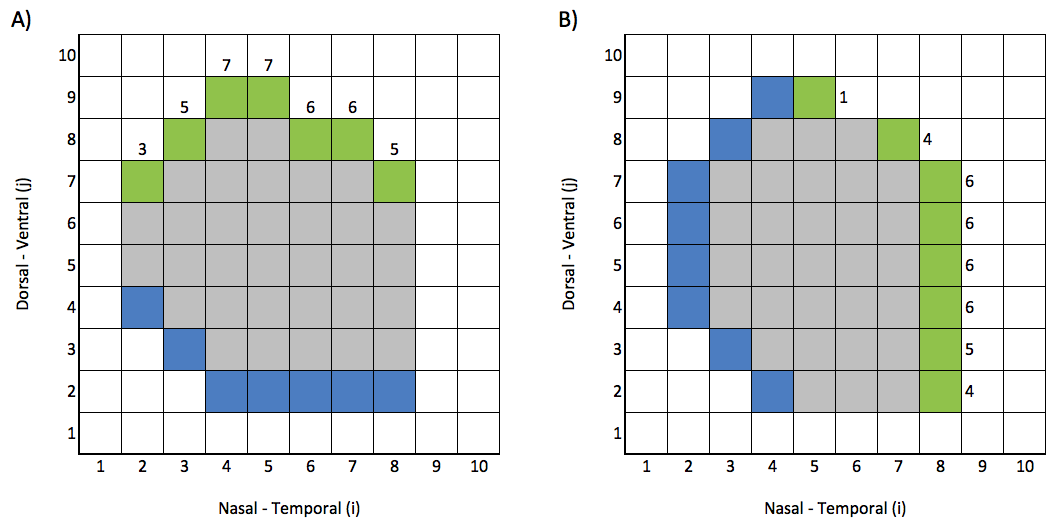
\includegraphics[scale=0.43]{AreaMethod}
\caption{\setstretch{1.0}\textbf{Scanning technique for receptive field area estimation.} Figures show the receptive field for a TC. Squares represent RGCs, filled squares indicate RGCs that synapse onto the TC. RF area is estimated using equation 12. 
\textbf{(A)} Scanning along the nasal-temporal axis of the retina. For each value of $i$: blue squares represent $jmin_i$, green squares represent $jmax_i$, numbers show $jmax_i - jmin_i$. Area estimate $= 3+5+7+7+6+6+5 = 39$
\textbf{(B)} Scanning along the dorsal-ventral axis of the retina. For each value of $j$: blue squares represent $imin_j$, green squares represent $imax_j$, numbers show $imax_j - imin_j$. Area estimate $= 1+4+6+6+6+6+5+4 = 38$.
Overall estimated area = $\frac{39 + 38}{2} = 38.5$
}
\end{figure}

\pagebreak

\begin{figure}[!h]
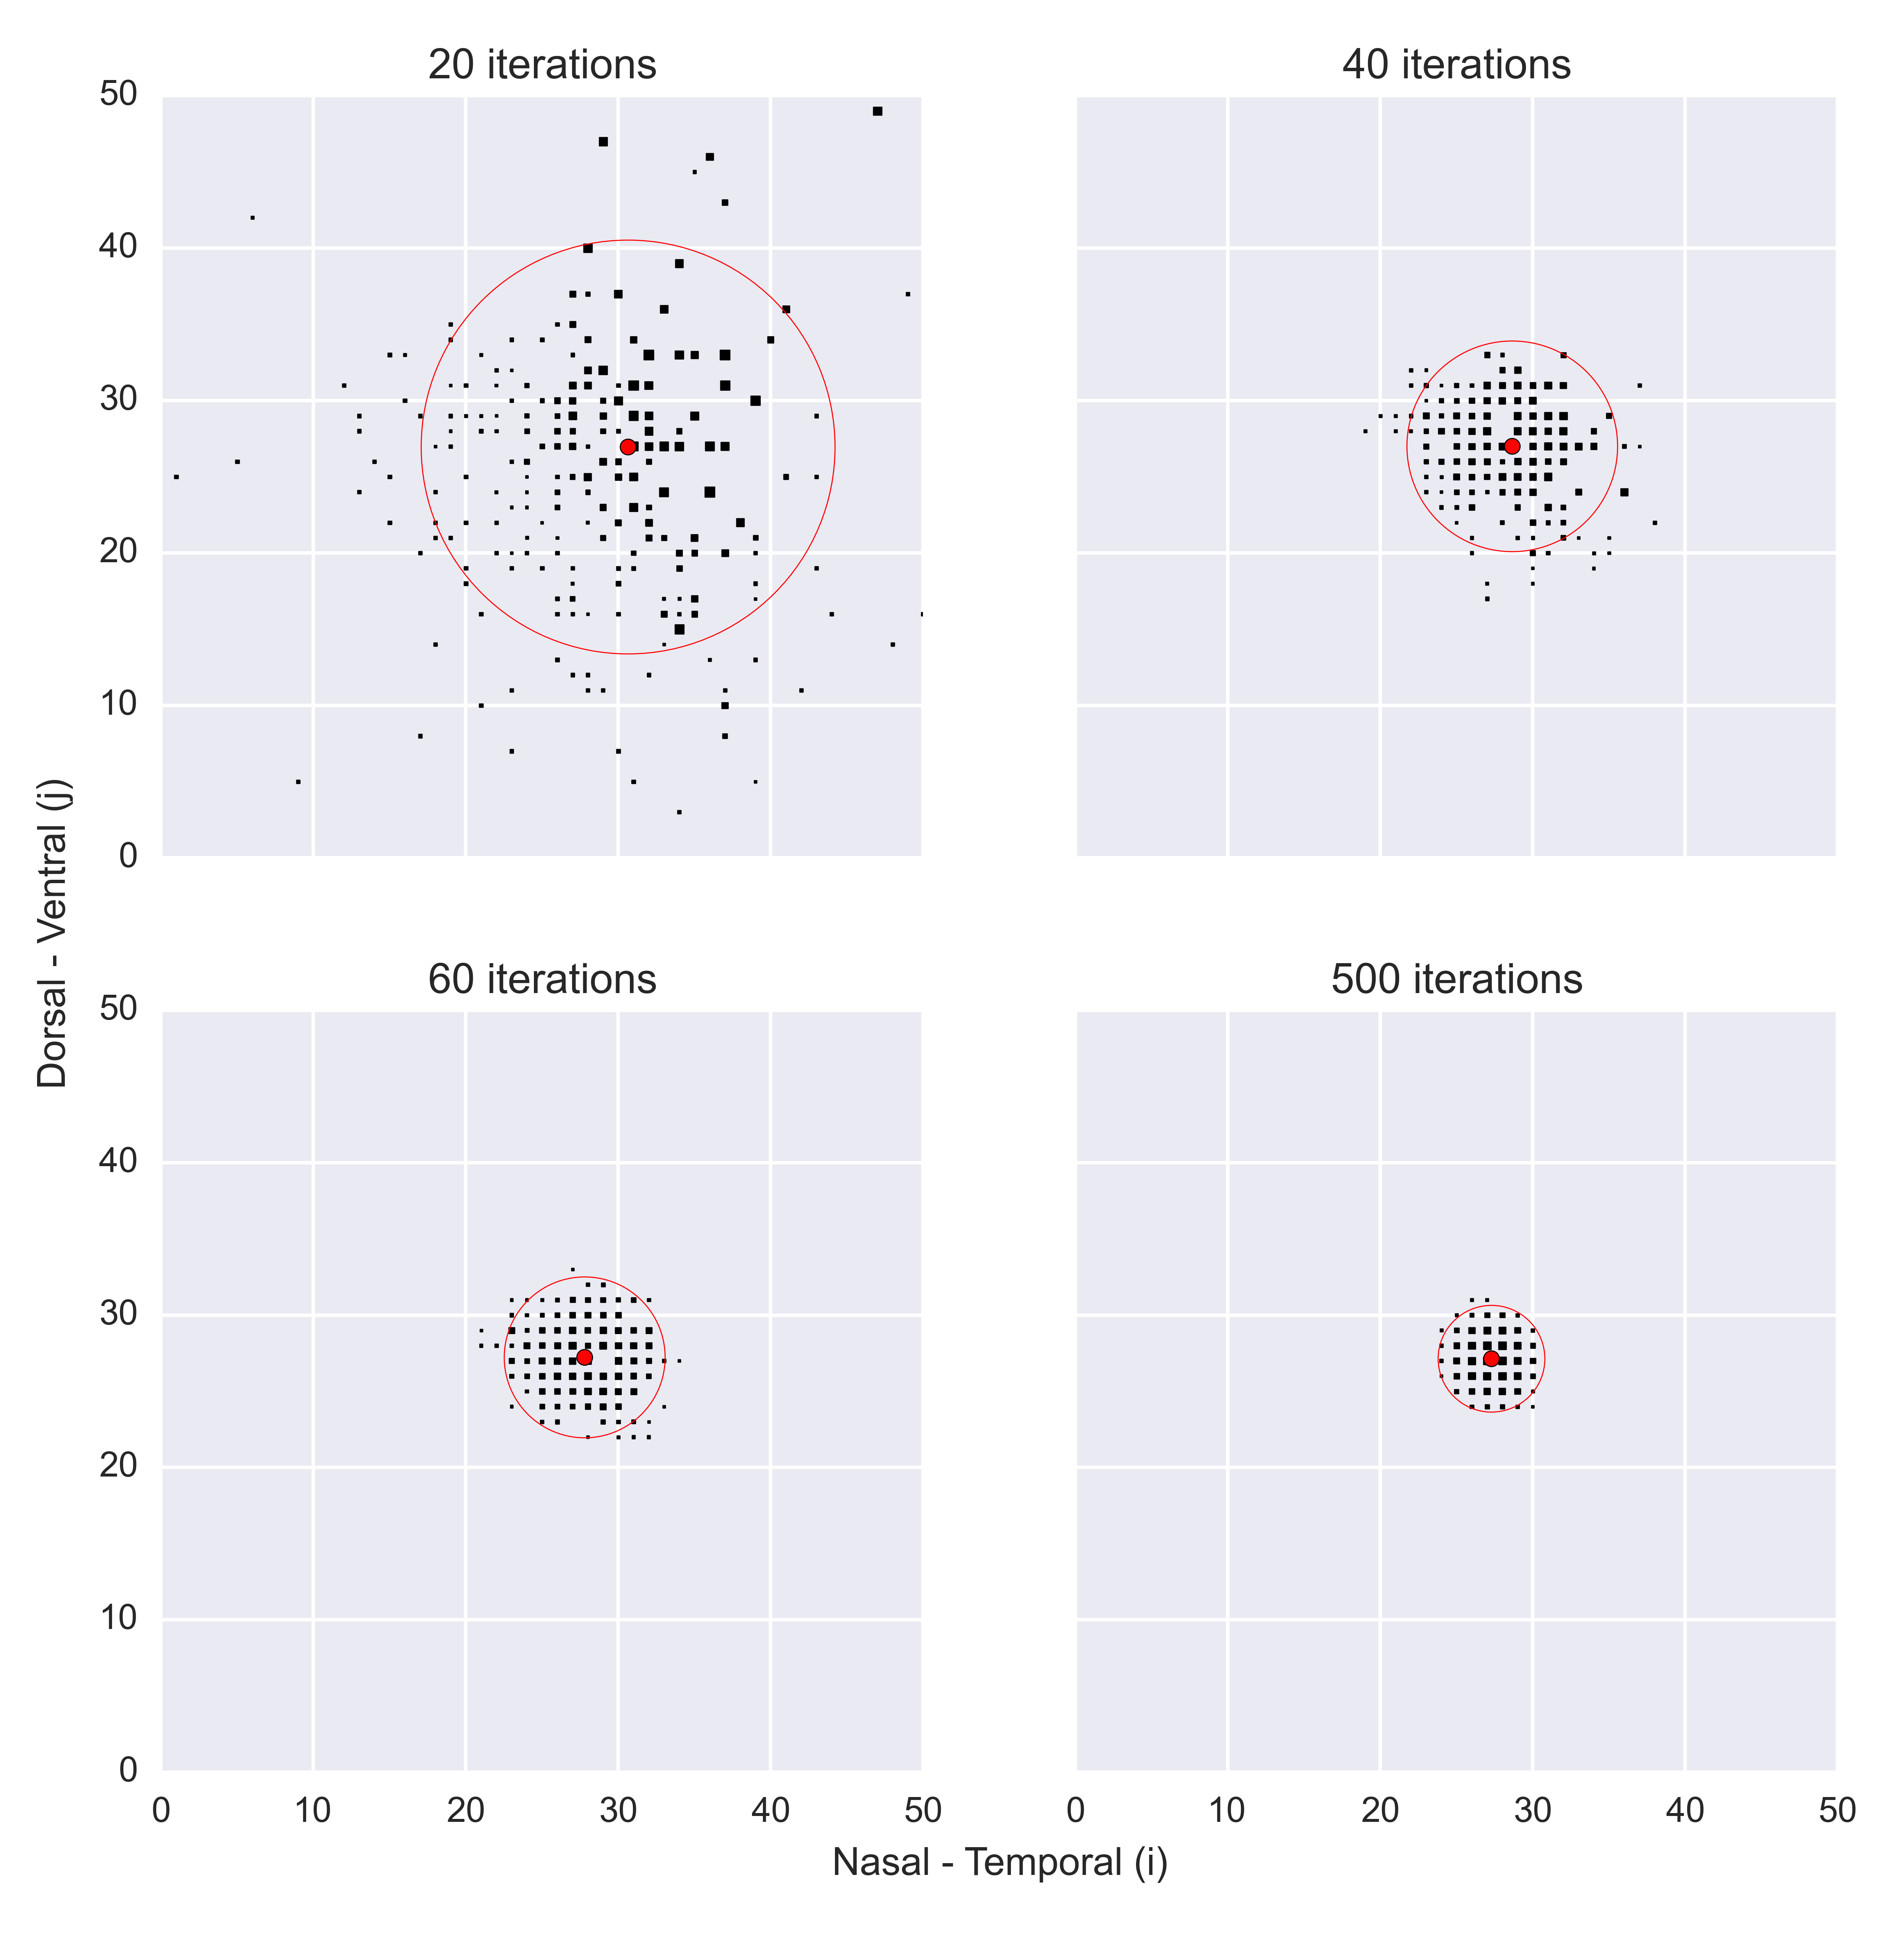
\includegraphics[scale=0.8]{AreaPlot}
\caption{\setstretch{1.0}\textbf{Examples of characterised receptive fields}. 
Figure shows the progression of the RF of a single TC at position $(25,25)$ over time throughout a regular simulation (50x50 retina and 50x50 tectum).
Points represent the presence of a synapse from an RGC at position $(i,j)$, point size represents synapse weight. Red circles indicate estimated RF circumference, and red dots indicate estimated RF centres. Estimated RF diameters for the four timepoints are, in order: 27.2, 13.8, 10.6 and 7.0}
\label{fig:AreaPlot}
\end{figure}

\pagebreak

\textbf{Map precision measurements}\\
In order to quantify the success of map formation I developed three measures of map precision, based on the characteristics of the RFs in the system:\\

\textbf{1) Mean receptive field separation:} the mean distance between the RF centres of adjacent TCs. The ideal map is an even, regular grid of RFs, where adjacent TCs have nearby RF centres in the retina. The optimum value will vary depending on the relative size of the retina and tectum, but assuming that they are of equal size, a value close to the distance separating TCs (1 unit) indicates that topography is set up in the system.
\\

\textbf{2) Mean receptive field diameter:} represents the acuity of the map. In successful maps, the overlap between RFs should be kept to a minimum, which is represented by a low value of this measure. A perfect map with 1:1 connections between the RGCs and TCs would have a mean RF diameter of 0.
\\

\textbf{3) Systems-match score:} the mean distance between the actual coordinates of the RF centres, and the coordinates that would be expected assuming perfect map formation. With an equal sized retina and tectum, given that maps should form in the correct orientation, RF coordinates in the form $(i,j)$ should be equal to TC coordinates in the form $(m,n)$ (i.e. $i = m$ and $j = n$). Given that the retina and tectum may not be of equal size, the expected RF centre coordinates for a TC ($xRF^c_{(m,n)}$) can be more generally written as equation 13, where $N_x$ represents the size of axis $x$, assuming that all axes are numbered from 1.

\begin{equation}
xRF^c_{(m,n)} = \left( m \frac{N_i}{N_m} , n \frac{N_j}{N_n} \right)
\end{equation}

The systems-match score is found by taking the mean of the distances between the actual RF centre and the expected RF centre for each TC. In a perfect map all RF centres should be at or close to their expected site, giving a systems-match score close to zero. Note that whilst an optimum mean RF separation score only requires maps to be topographic, an optimum mean systems-match score requires maps to be in the correct location and orientation. Therefore, consideration of both measures allows for separate assessment of topography and map placement.\\

In order to eliminate the effect of boundaries, which distort maps at their edges, I excluded a 5 cell thick ring of cells at the boundary of the tectum from all precision calculations. This therefore limits these measures to the inner TCs that are isolated from the boundaries.\\


\subsection{Programming}
All programming was performed in Python. The package NumPy was used to perform  calculations in the model. The packages Matplotlib and Seaborn were used to create figures. All Python code used in the project is new and was written independently. Code can be found online at \texttt{github.com/tsmbland/RetinotopicMaps}, along with instructions for performing simulations.\\


\section{Results}

\subsection{Normal Map Progression}

I begin by demonstrating the performance of the model in a normal development simulation. In these simulations a 50x50 retina and 50x50 tectum are used, which are kept at a constant size throughout, and ran for up to 20,000 iterations. Initial gradients are set as in figure 5. Resulting maps are best visualised using a lattice plot (figure 8) which represents a projection of the tectum onto the retina. This shows that, starting with an initial random pattern of connections, global topographic order develops, with adjacent TCs receiving inputs from adjacent regions of the retina.\\


\begin{figure}[!h]
\includegraphics[scale=0.6]{Fieldplots}
\caption{\setstretch{1.0}\textbf{Map progression over time.} 
Plots show a map of the tectum projected onto the retina (represented by the grey background). Nodes in lattices represent individual TCs, and the location of a node represents its RF centre coordinates. Links connect RF centres of directly adjacent TCs. This figure shows that, starting with a random pattern of connections, ordered maps develop over time.}
\end{figure}

\pagebreak

Analysis of my three precision measures over time (figure 9) gives an insight into the sequence of events in map formation. Early phases in development are characterised by a rapid fall in mean RF separation, indicating that topography is rapidly set up. This coincides with a rapid decline in mean RF size, representing an increase in map acuity. The systems-match score also displays a short phase of rapid decline, but follows this with a prolonged phase of slower decline, approximately halving in value between iterations 1,000 and 5,000, stabilising close to the optimum score of 0. This suggests that the map undergoes a more prolonged phase of placement and orientation correction after topography is set up. The low final value confirms that the map is in the correct orientation and position.\\

\begin{SCfigure}[][!h]
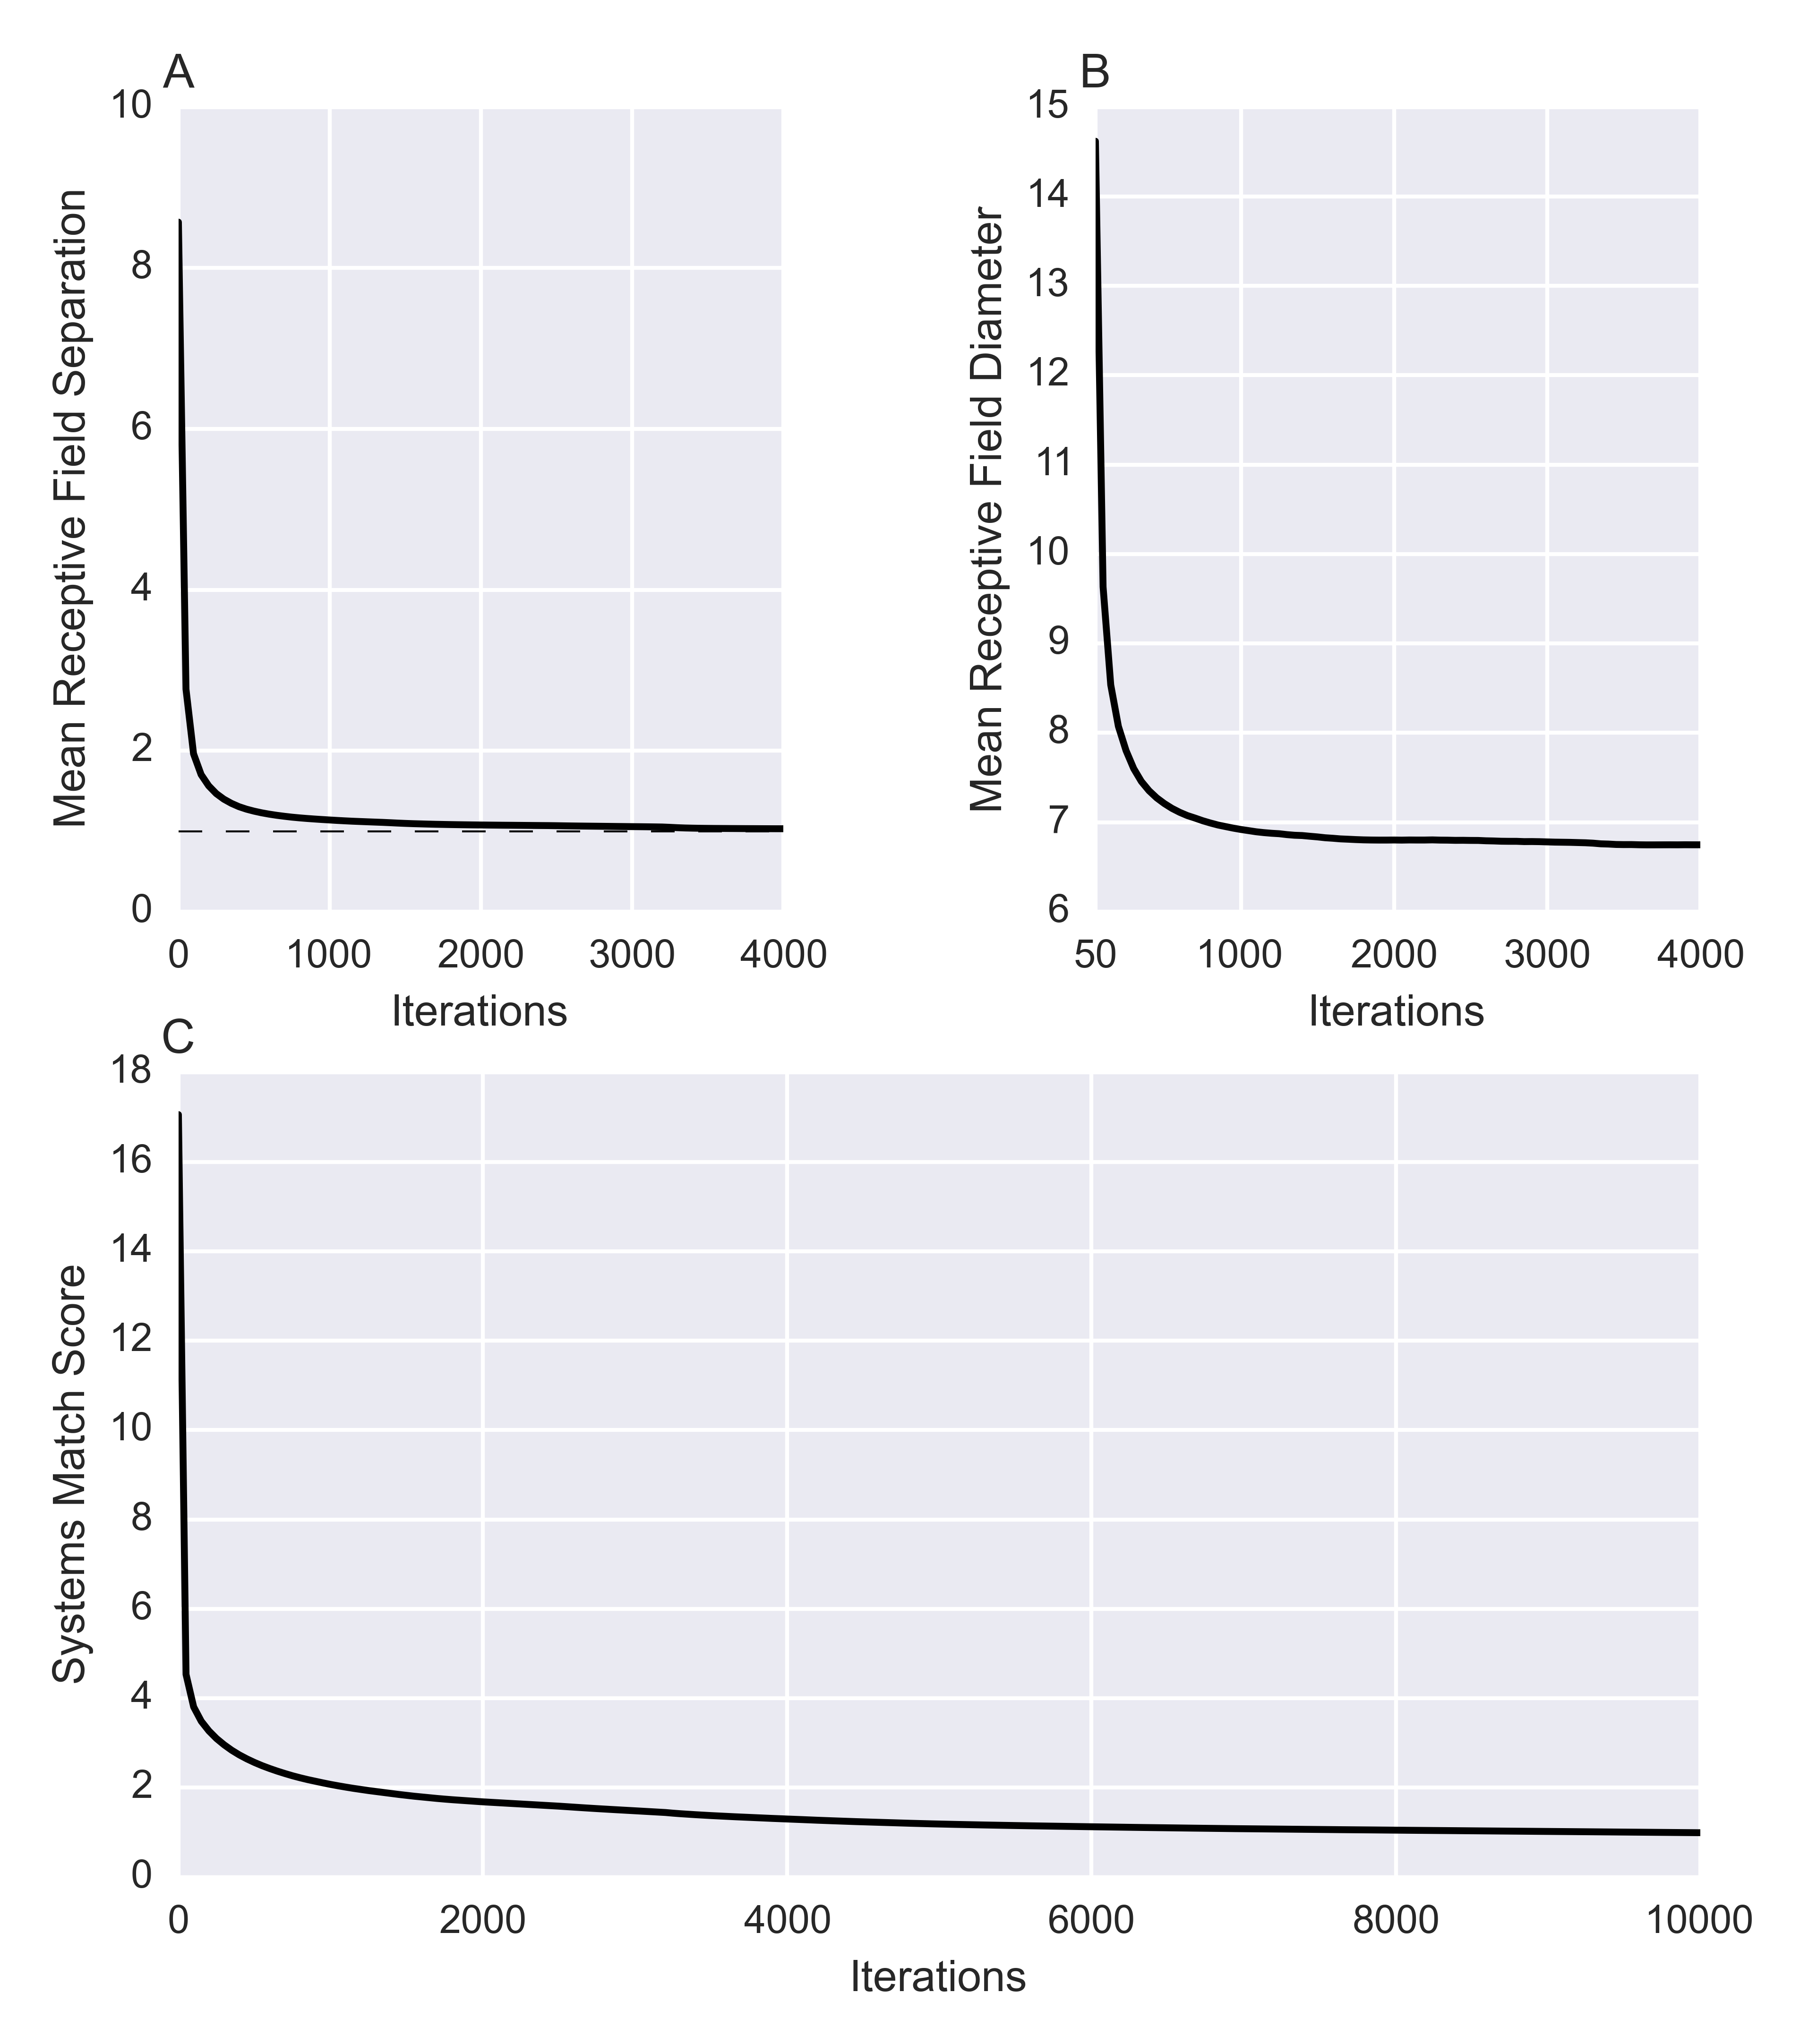
\includegraphics[scale=0.67]{PrecisionPlot}
\caption{\setstretch{1.0}\textbf{Precision of the map over time.}
Figure shows how my three precision measures change over time during a normal simulation.
\textbf{(A)} Mean RF separation displays rapid decline, stabilising close to its theoretical optimum level (indicated by the dashed line).
\textbf{(B)} Mean RF diameter displays rapid decline and stabilisation. 
Data shown from iteration 50 onwards to exclude unreliable estimates at early times when connections are sparse and RFs noncircular.
\textbf{(C)} Systems-match score displays a phase of rapid decline, and a more prolonged phase of slower decline, before eventual stabilisation close to the optimum score of zero.}
\end{SCfigure}

\pagebreak

\subsection{Mismatch Surgery}
Mismatch experiments were instrumental in the initial proposal of the marker-induction model, providing key evidence for map plasticity. Whilst the original 1979 model showed a good ability to recapitulate results from experimental studies, these studies have not been revisited since the marker-induction model was updated in 2006, and there currently lacks any report of a two-dimensional Eph/ephrin marker-induction model undergoing similar operations. I therefore subjected my up to date model to a number of virtual surgery operations, and tested for its ability to predict the qualitative findings of the original experimental studies. Three experimental observations were tested:\\

1) A half-retina can form an expanded map over the entire tectum (Schmidt et al., 1978)

2) A whole retina can form a compressed map over a half-tectum (Gaze and Sharma, 1970)

3) A half-retina can form a map over a foreign half-tectum (Horder, 1971)\\

Figure 10 shows examples of simulations performing surgery in the dimensions of the Eph/ephrinA system. In all cases the model generates maps that match qualitatively with the experimental observations. Surgery in the Eph/ephrinB system dimensions was also simulated, and gave similar results.


\pagebreak
\begin{figure}[!h]
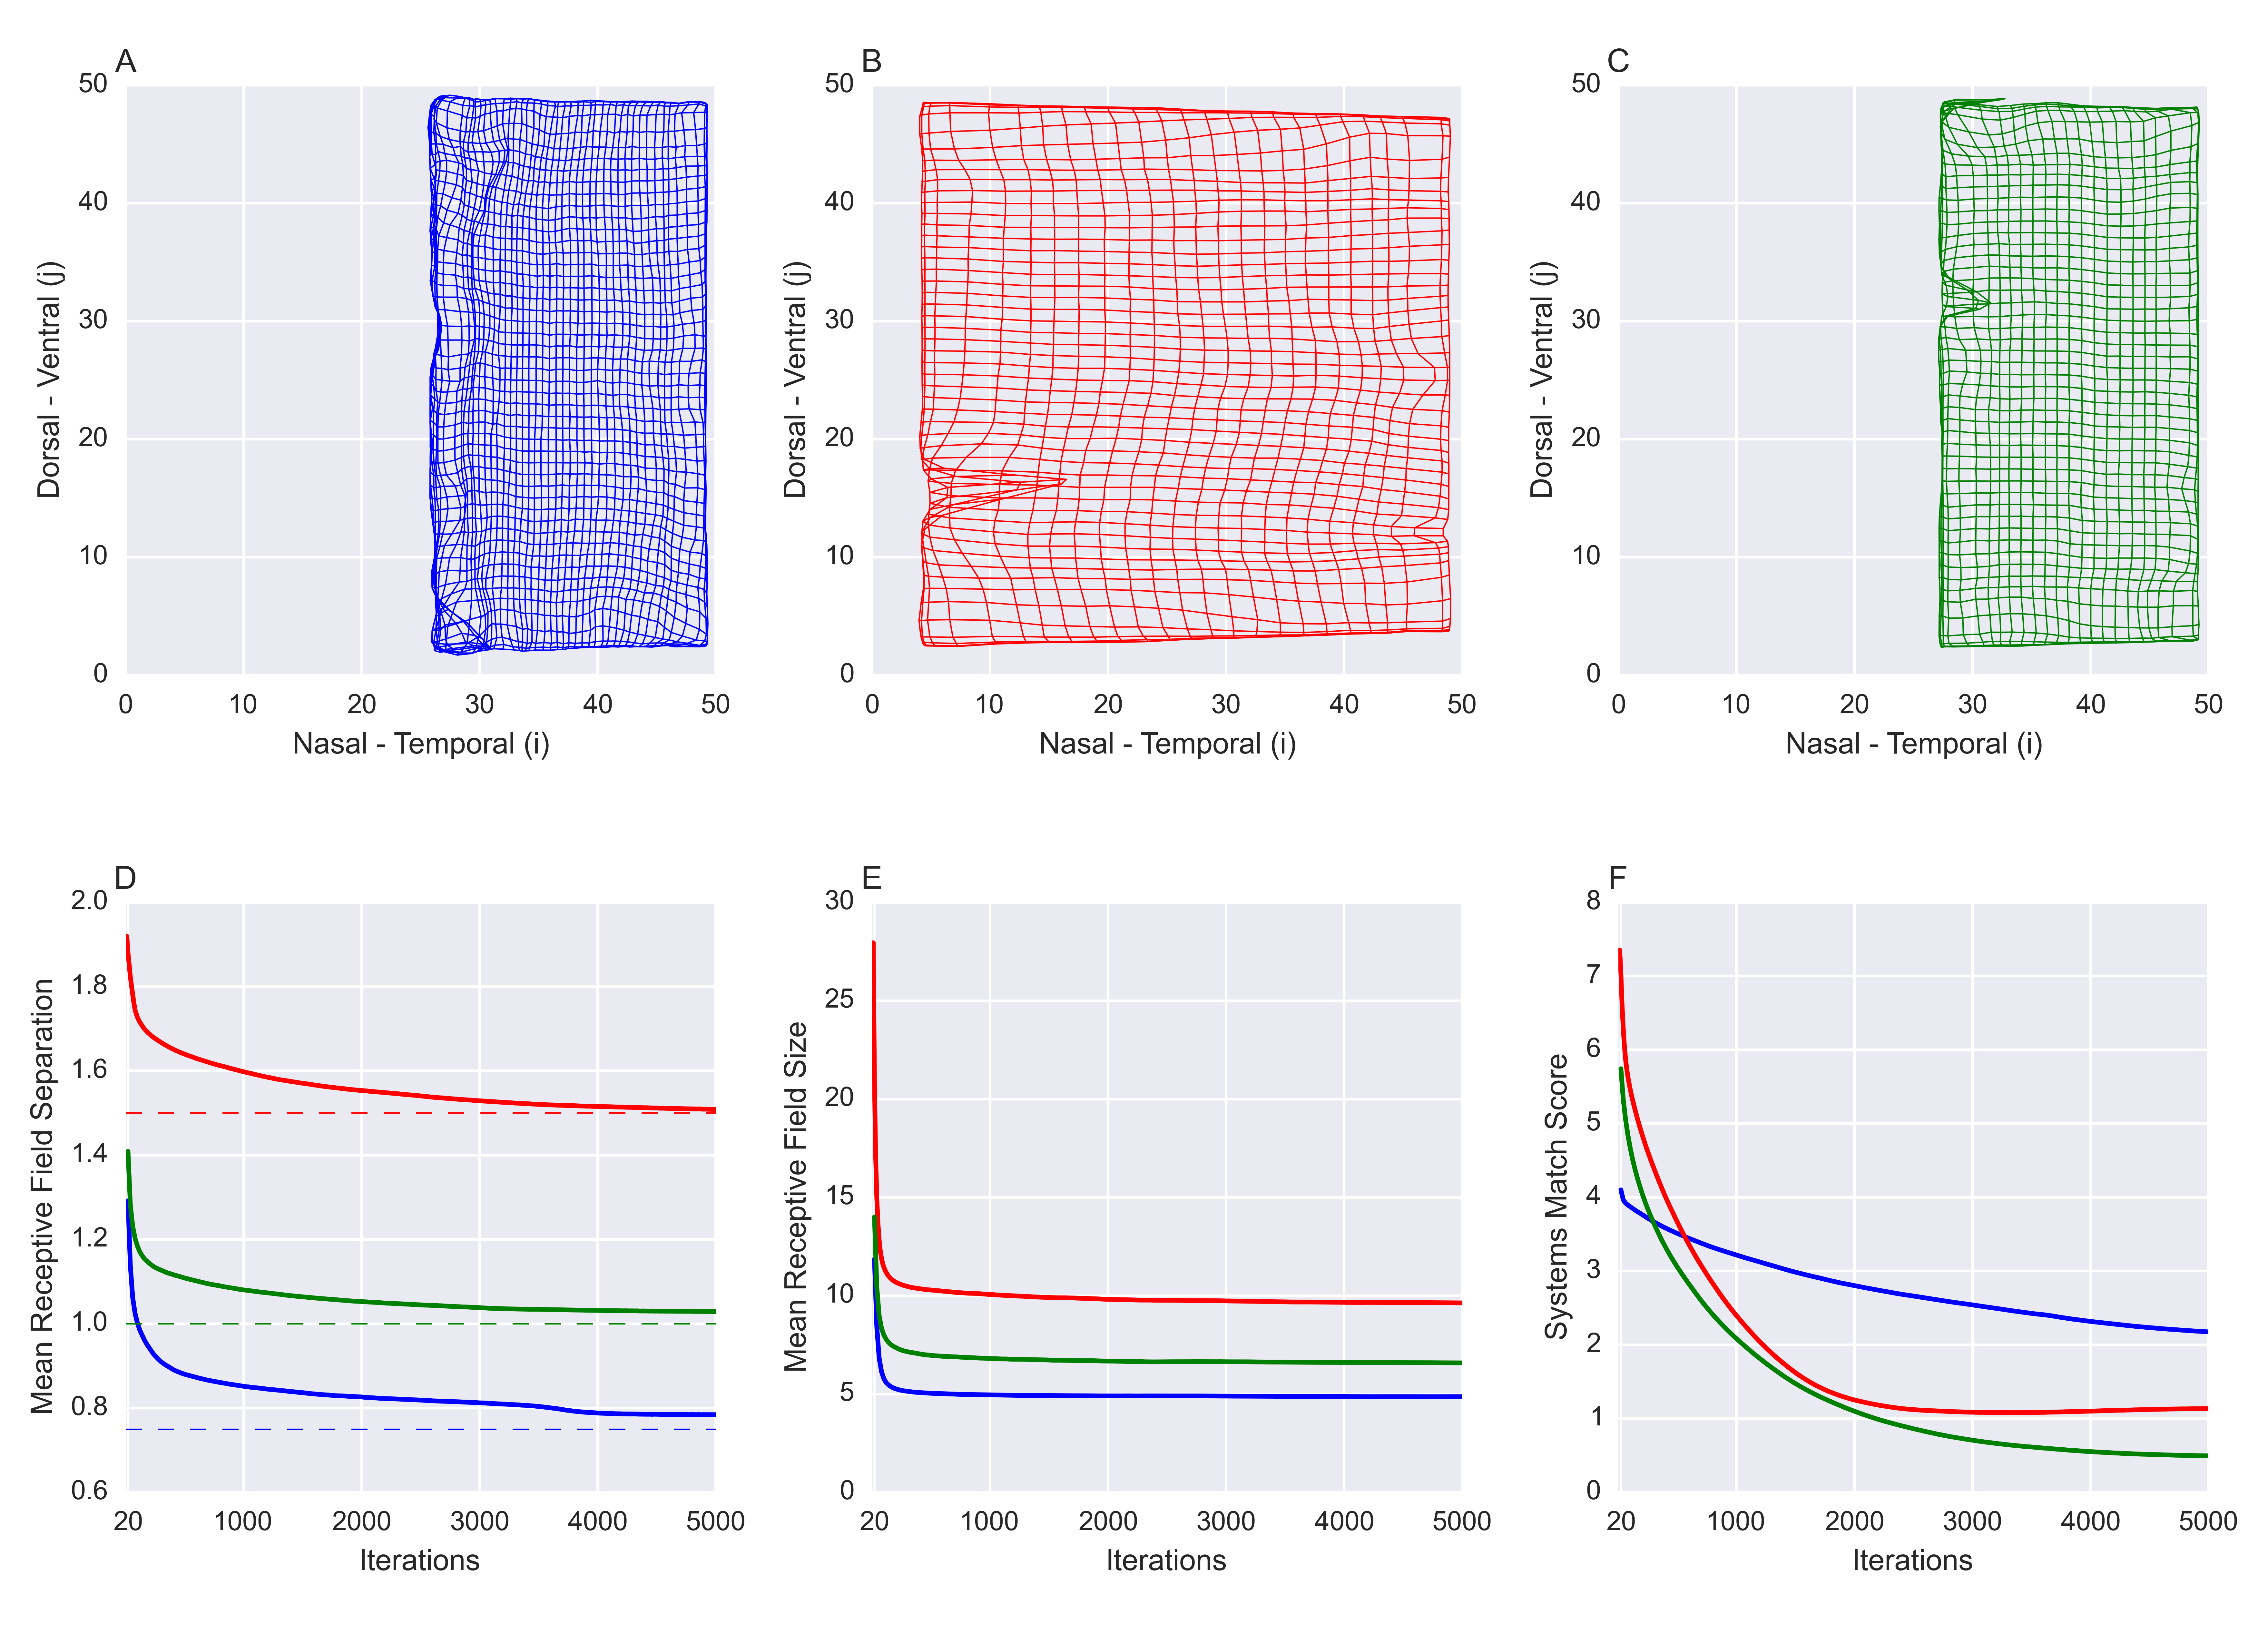
\includegraphics[scale=0.55]{SurgeryPlot}
\caption{\setstretch{1.0}\textbf{Maps generated after three different surgery operations.} Simulations were set up to correspond with a typical mismatch surgery experiment. Full size maps (50x50 retina and 50x50 tectum) were first allowed to develop normally and reach a steady state (20,000 iterations). Synaptic weight matrices were then reset to zero, simulating cutting of the optic nerve. A group of cells was then removed from the retina and/or tectum, and the remaining RGCs allowed to connect randomly to the remaining part of the tectum. Simulations then proceeded as normal, and precision measures were follwed. 
\textbf{(A) - (C)} Lattice plots showing a map of the tectum projected onto the retina at the end of 5,000-iteration simulations.
(A) Surgery 1: Map of a whole tectum on a half retina (temporal half).
(B) Surgery 2: Map of a half tectum (posterior half) on a whole retina.
(C) Surgery 2: Map of a half tectum (posterior half) onto the foreign half of the retina (temporal half).
\textbf{(D) - (F)} Map precision measures over time for the three simulations, shown from iteration 20 onwards. Line colours correspond to map colours in (A) - (C). Dashed lines in (D) represent the theoretical optimum RF separation for each simulation. Measures show that where the retina and tectum are a different size (surgeries 1 and 2), maps are correctly compressed or expanded (D), with a corresponding change in receptive field sizes (E). Systems-matching is slightly impaired (F), but not far from optimum. Where the retina and tectum are the same size (surgery 3), results match closely with the normal development scenario presented in section 3.1.}
\end{figure}
\pagebreak

\subsection{Manipulation of Retinal Gradients}
A number of genetic studies of retinotopic map formation, manipulating retinal and tectal Eph and ephrin gradients, have been performed in mice (Brown et al., 2000; Feldheim et al., 2000; Reber et al., 2004). Any valid model of map formation should be able to recapitulate the phenotypes that these manipulations bring about. A specific well-described genetic manipulation is the knockin of the \textit{EphA3} gene in the retina of mice (Brown et al., 2000). Approximately half of all RGCs, by random, express the \textit{Islet2} gene. Insertion of \textit{EphA3} cDNA (which is not normally expressed in RGCs) into the \textit{Islet2} gene raises the total EphA density in these cells, effectively creating two distinct EphA gradients across the nasal-temporal axis of the retina. In these mice the outcome is two separate ordered projections of the retina onto the SC from the two cell populations (figure 11). The fact that \textit{EphA3}$^+$ cells form an ordered map provides support for the marker-induction model, by showing that RGC to SC cell connections can form even when retinal Eph densities are raised above their normal physiological levels. This is explained in the marker-induction model by a corresponding change in anterior SC gradients.\\

\begin{SCfigure}[][!h]
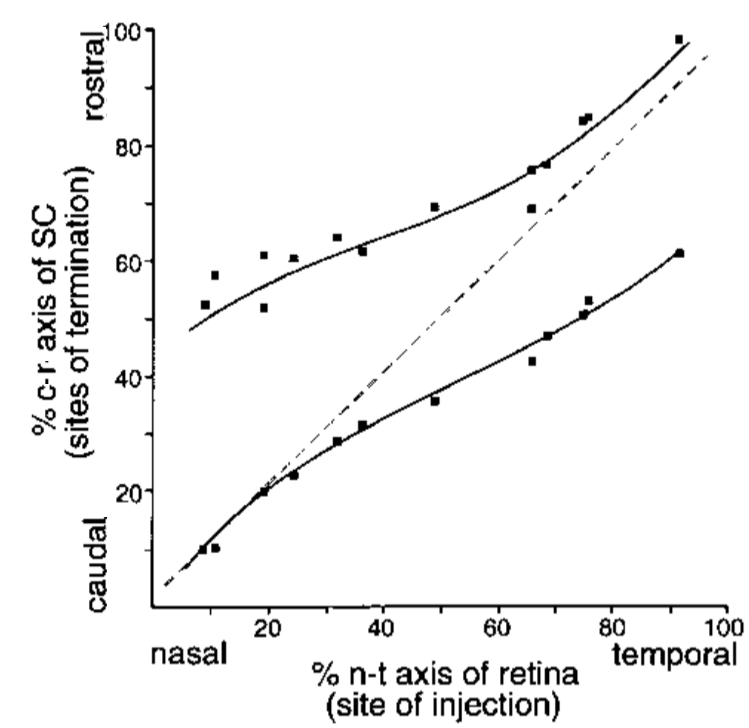
\includegraphics[scale=0.3]{Brown}
\caption{\setstretch{1.0}\textbf{Double projection in \textit{EphA3}-knockin mice.}
Connection pattern between a one-dimensional slice of cells across the retina and a one-dimensional slice of cells across the SC. Points show the presence of a connection between an RGC and an SC cell. The connection pattern can be described by two approximately linear curves, representing the two RGC populations, the more rostral curve representing the \textit{EphA3}$^+$ population. The dashed line indicates the connection pattern in wild type mice. Caudal and rostral are referred to in this report as posterior and anterior respectively. Figure adapted from Brown et al. (2000)}
\end{SCfigure}

\pagebreak

In its original analysis, the 2006 marker-induction model demonstrated a good ability to predict these findings. I performed a similar analysis with my new model. \textit{EphA3}-knockin was simulated by randomly raising EphA density by a constant in half of all RGCs (figure 12A). Maps were then allowed to develop normally with these retinal EphA densities. The model successfully recapitulates the experimental observations, forming two distinct maps (figures 12B and C).\\


\begin{figure}[!h]
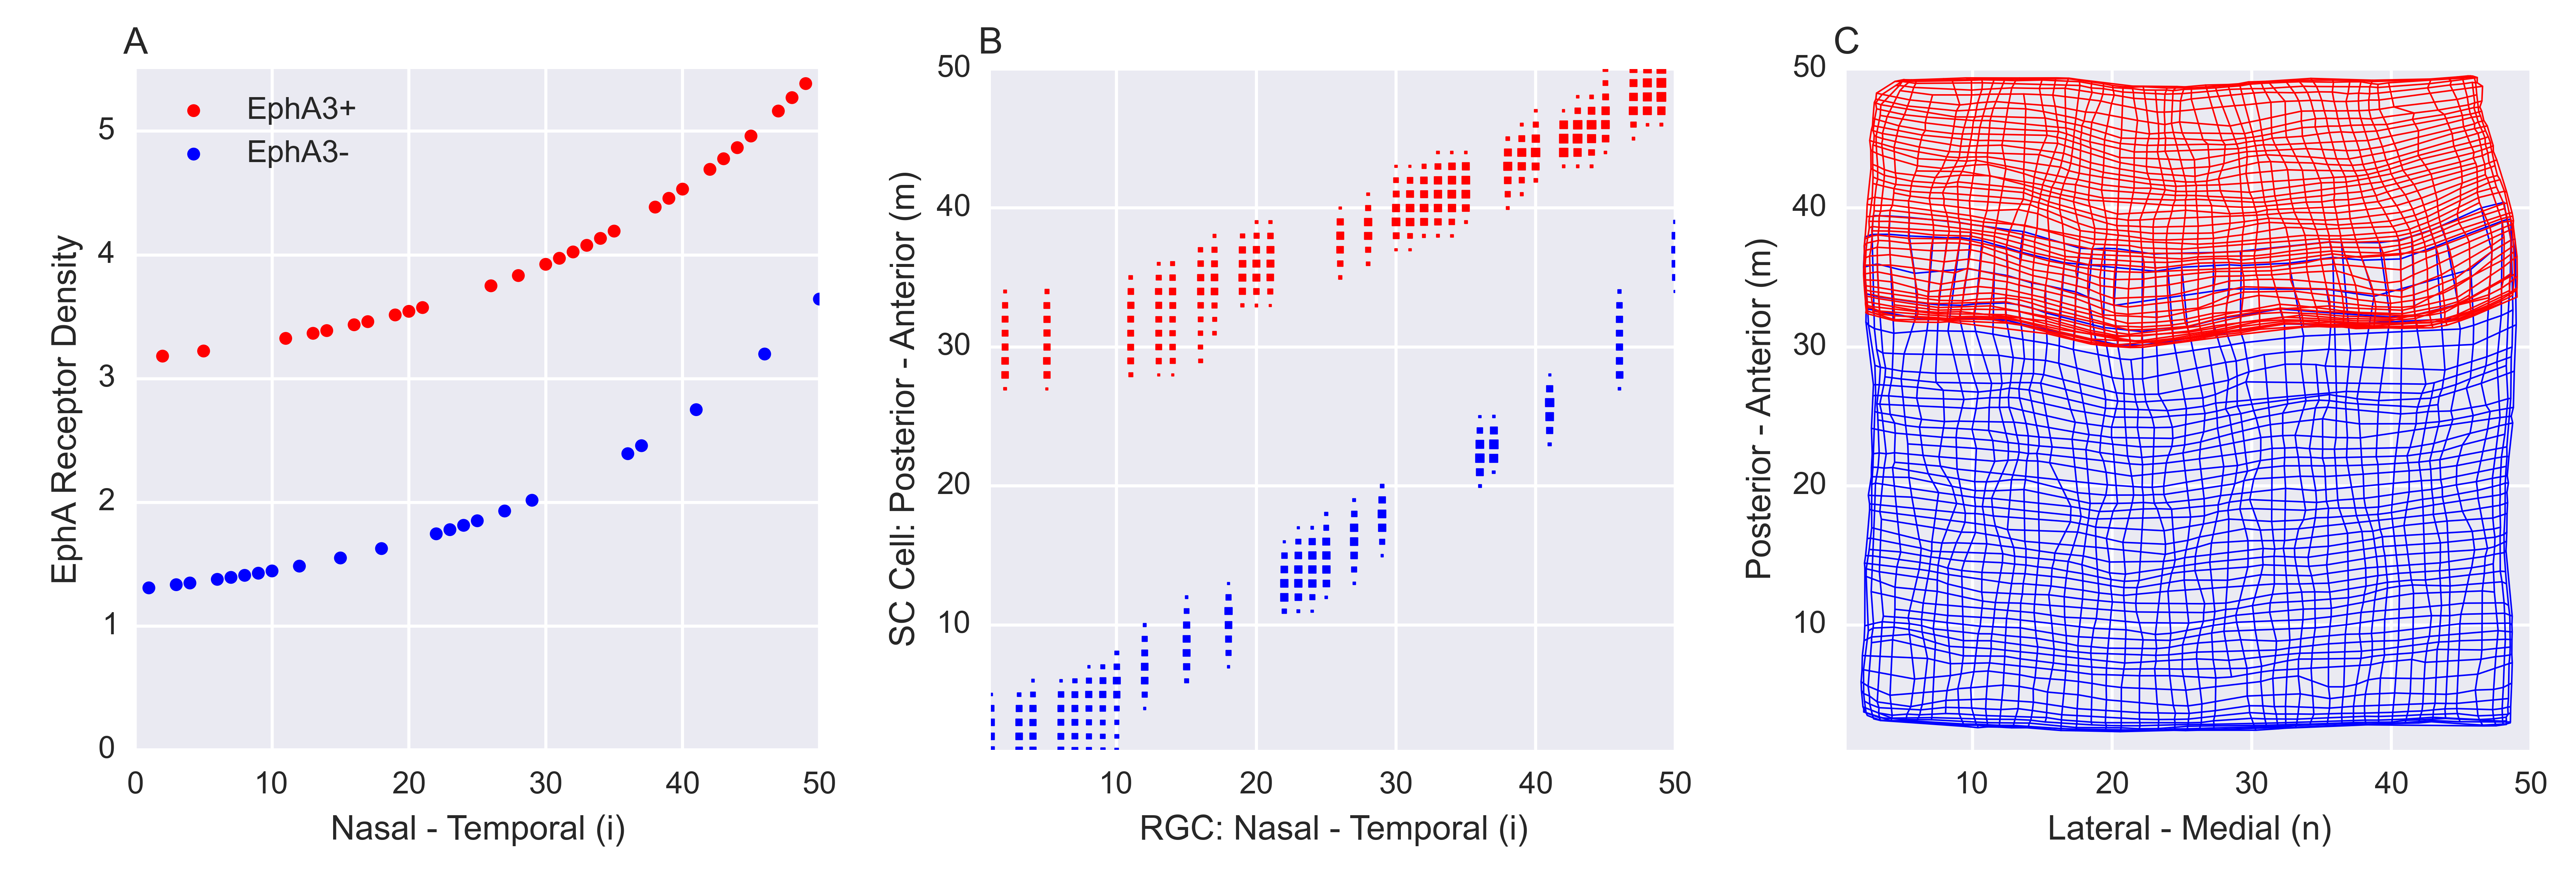
\includegraphics[scale=0.57]{EphA3}
\caption{\setstretch{1.0}\textbf{\textit{EphA3}-knockin simulation.}
\textbf{(A)} EphA receptor density profile across the nasal-temporal axis of the retina. Cells were randomly assigned with equiprobability as \textit{EphA3}$^+$ (red) or \textit{EphA3}$^-$ (blue). \textit{EphA3}$^-$ cells follow the normal gradient shown in figure 5A. \textit{EphA3}$^+$ cells are given an additional 1.86 EphA receptor density units. 
\textbf{(B)} Connection pattern between a one-dimensional slice of cells across the retina and a one-dimensional slice of cells across the SC, analogous to the experimental data in figure 11. Slices were taken half way along the orthogonal axes. Points indicate a synapse, point size indicates synaptic weight. As with the experimental data, two distinct projections can be seen from the \textit{EphA3}$^+$ (red) and \textit{EphA3}$^-$ (blue) cells.
Plot shows a stable connectivity pattern after 10,000 iterations.
\textbf{(C)} Two-dimensional lattice plot showing a map of the retina projected onto the SC. Nodes in lattices represent individual RGCs, and the location of a node represents its PF centre coordinates. Links connect PF centres of directly adjacent RGCs. Projections of \textit{EphA3}$^+$ (red) and \textit{EphA3}$^-$ (blue) cells are shown separately. Two separate maps are formed from the two cell types, with the \textit{EphA3}$^+$ map more anterior than the \textit{EphA3}$^-$ map. Plot shows a stable projection after 10,000 iterations.}
\end{figure}
\pagebreak

\subsection{Manipulation of Tectal Gradients}


Whilst the need for some initial tectal gradients is well understood, there is currently very little quantitative information about the strength of these gradients. I attempted to predict the minimum amount of tectal information required to permit ordered maps by testing my model with initial tectal gradients of varying strength, set by multiplying default gradients (figure 5C-D) by a scaling factor, ranging from 0 to 1. Predictions can be compared to real measurements of tectal ephrin gradients, when they become available, in order to assess the feasibility of the model and its parameter set.
\\

Results (figure 13) show that as tectal information decreases, map precision gets worse, as would be expected. There appears to be a rough threshold, with all three measures little affected until gradients are scaled down to below around 0.6x their default value, and rapidly increasing after this. This therefore represents the predicted minimum required tectal gradient. 
\\

\begin{figure}[!h]
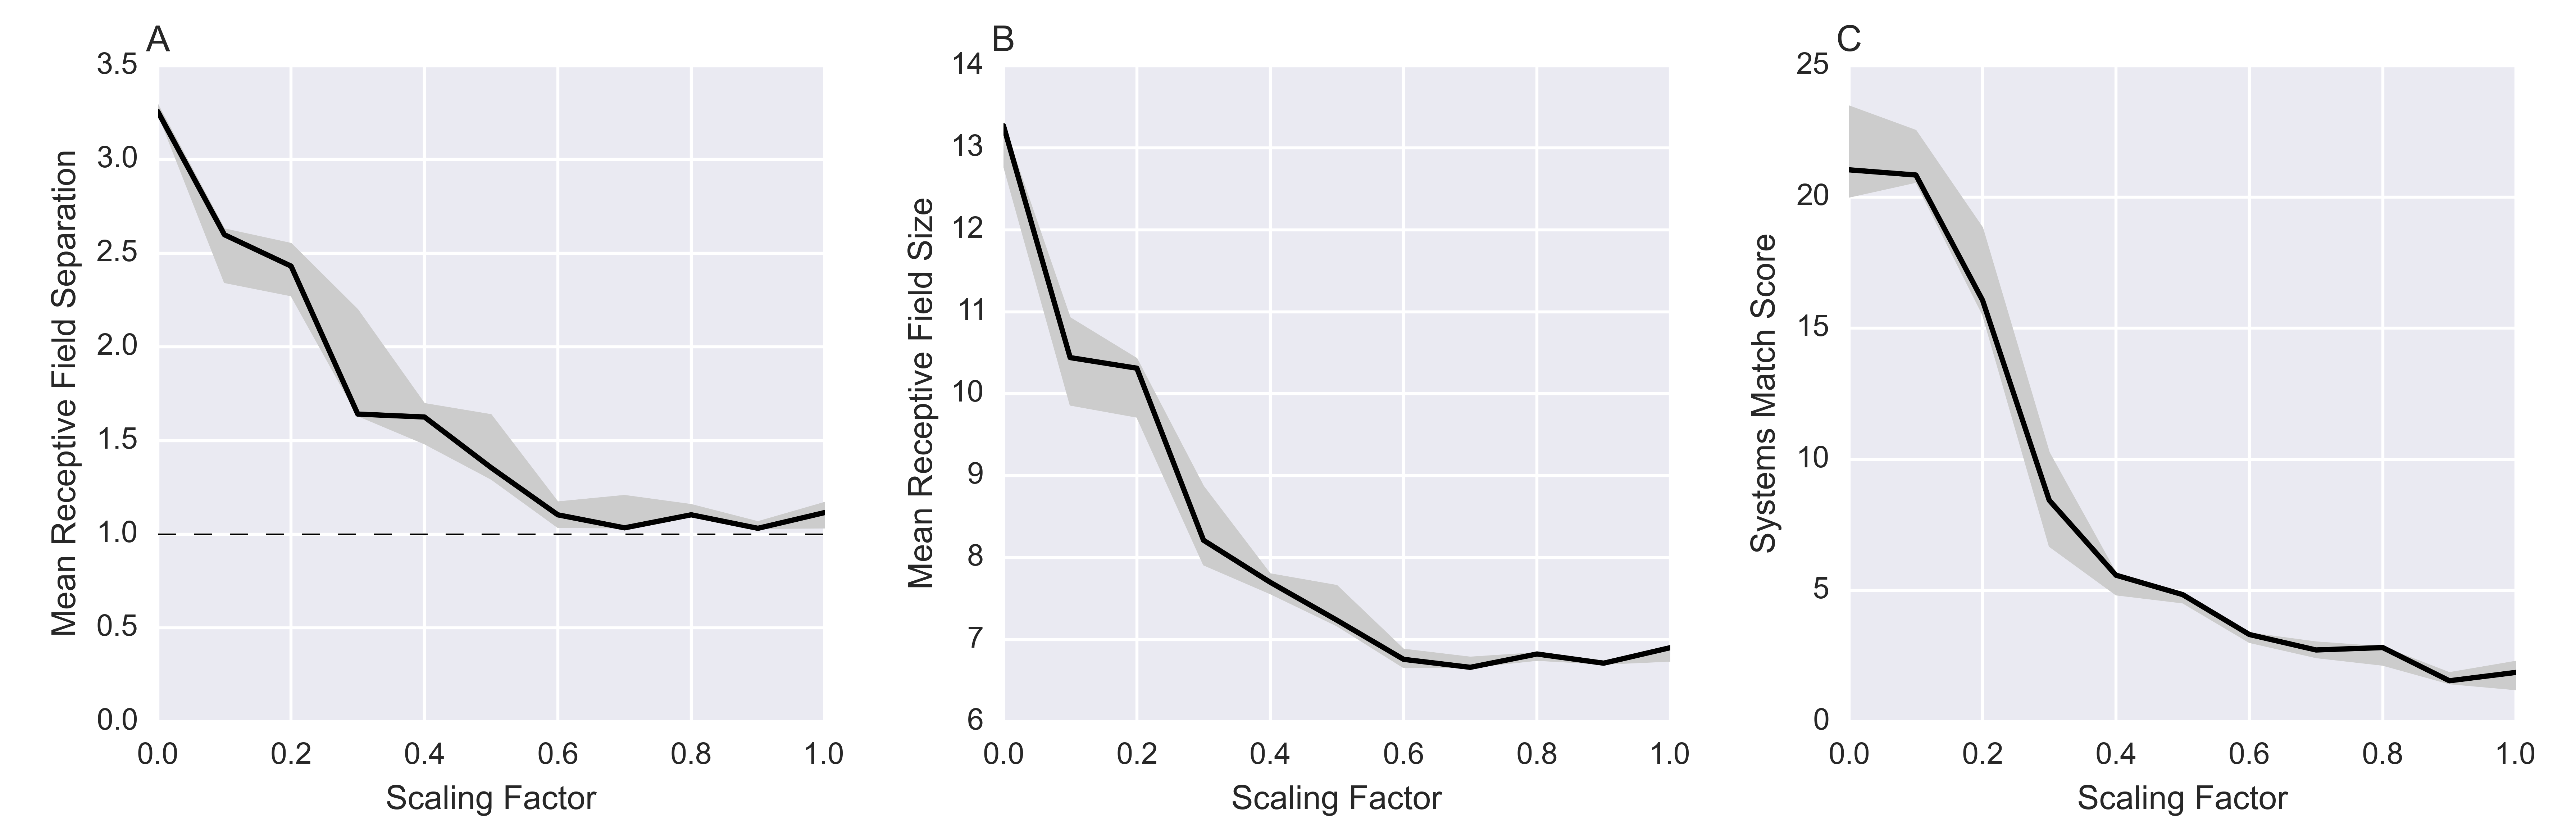
\includegraphics[scale=0.55]{TectalInfoPlot}
\caption{\setstretch{1.0}\textbf{The influence of initial tectal information on final map precision.}
Tectal gradients were set by multiplying the default gradients shown in figure 5C-D by the scaling factor. Three simulations were performed for each tectal gradient in a 50x50 retina and 50x50 tectum system, and precision measures taken after 5,000 iterations. Black lines show median results, shaded areas are bounded by the maximum and minimum results. Dashed line in (A) represents the theoretical optimum. NB the mean RF separation expected in totally disordered maps (calculated as the mean score across all trials at at time $=$ 0, when connection patterns are completely random) is 8.5, indicating that there is some degree of refinement even in the absence of any tectal information.}
\end{figure}

\pagebreak

\subsection{Model Performance Comparison}
As explained in section 2.1, the changes that I made to the model were predicted to increase computational performance. In order to assess these improvements, I ran my reproduction of the 2006 model and my new model for a range of system sizes, and compared simulation running times. Both models underwent the same optimisation protocol, and differed only in their interpretation of synapses. The results (figure 14) show a dramatic improvement in larger systems, with a roughly 8.5x speed increase in the largest systems tested. Simulation speed is important as it determines the maximum system size that can be feasibly simulated. For example, for the same running time, systems can be scaled up from 30 cells/dimension to over 50 cells/dimension.

\begin{SCfigure}[][h]
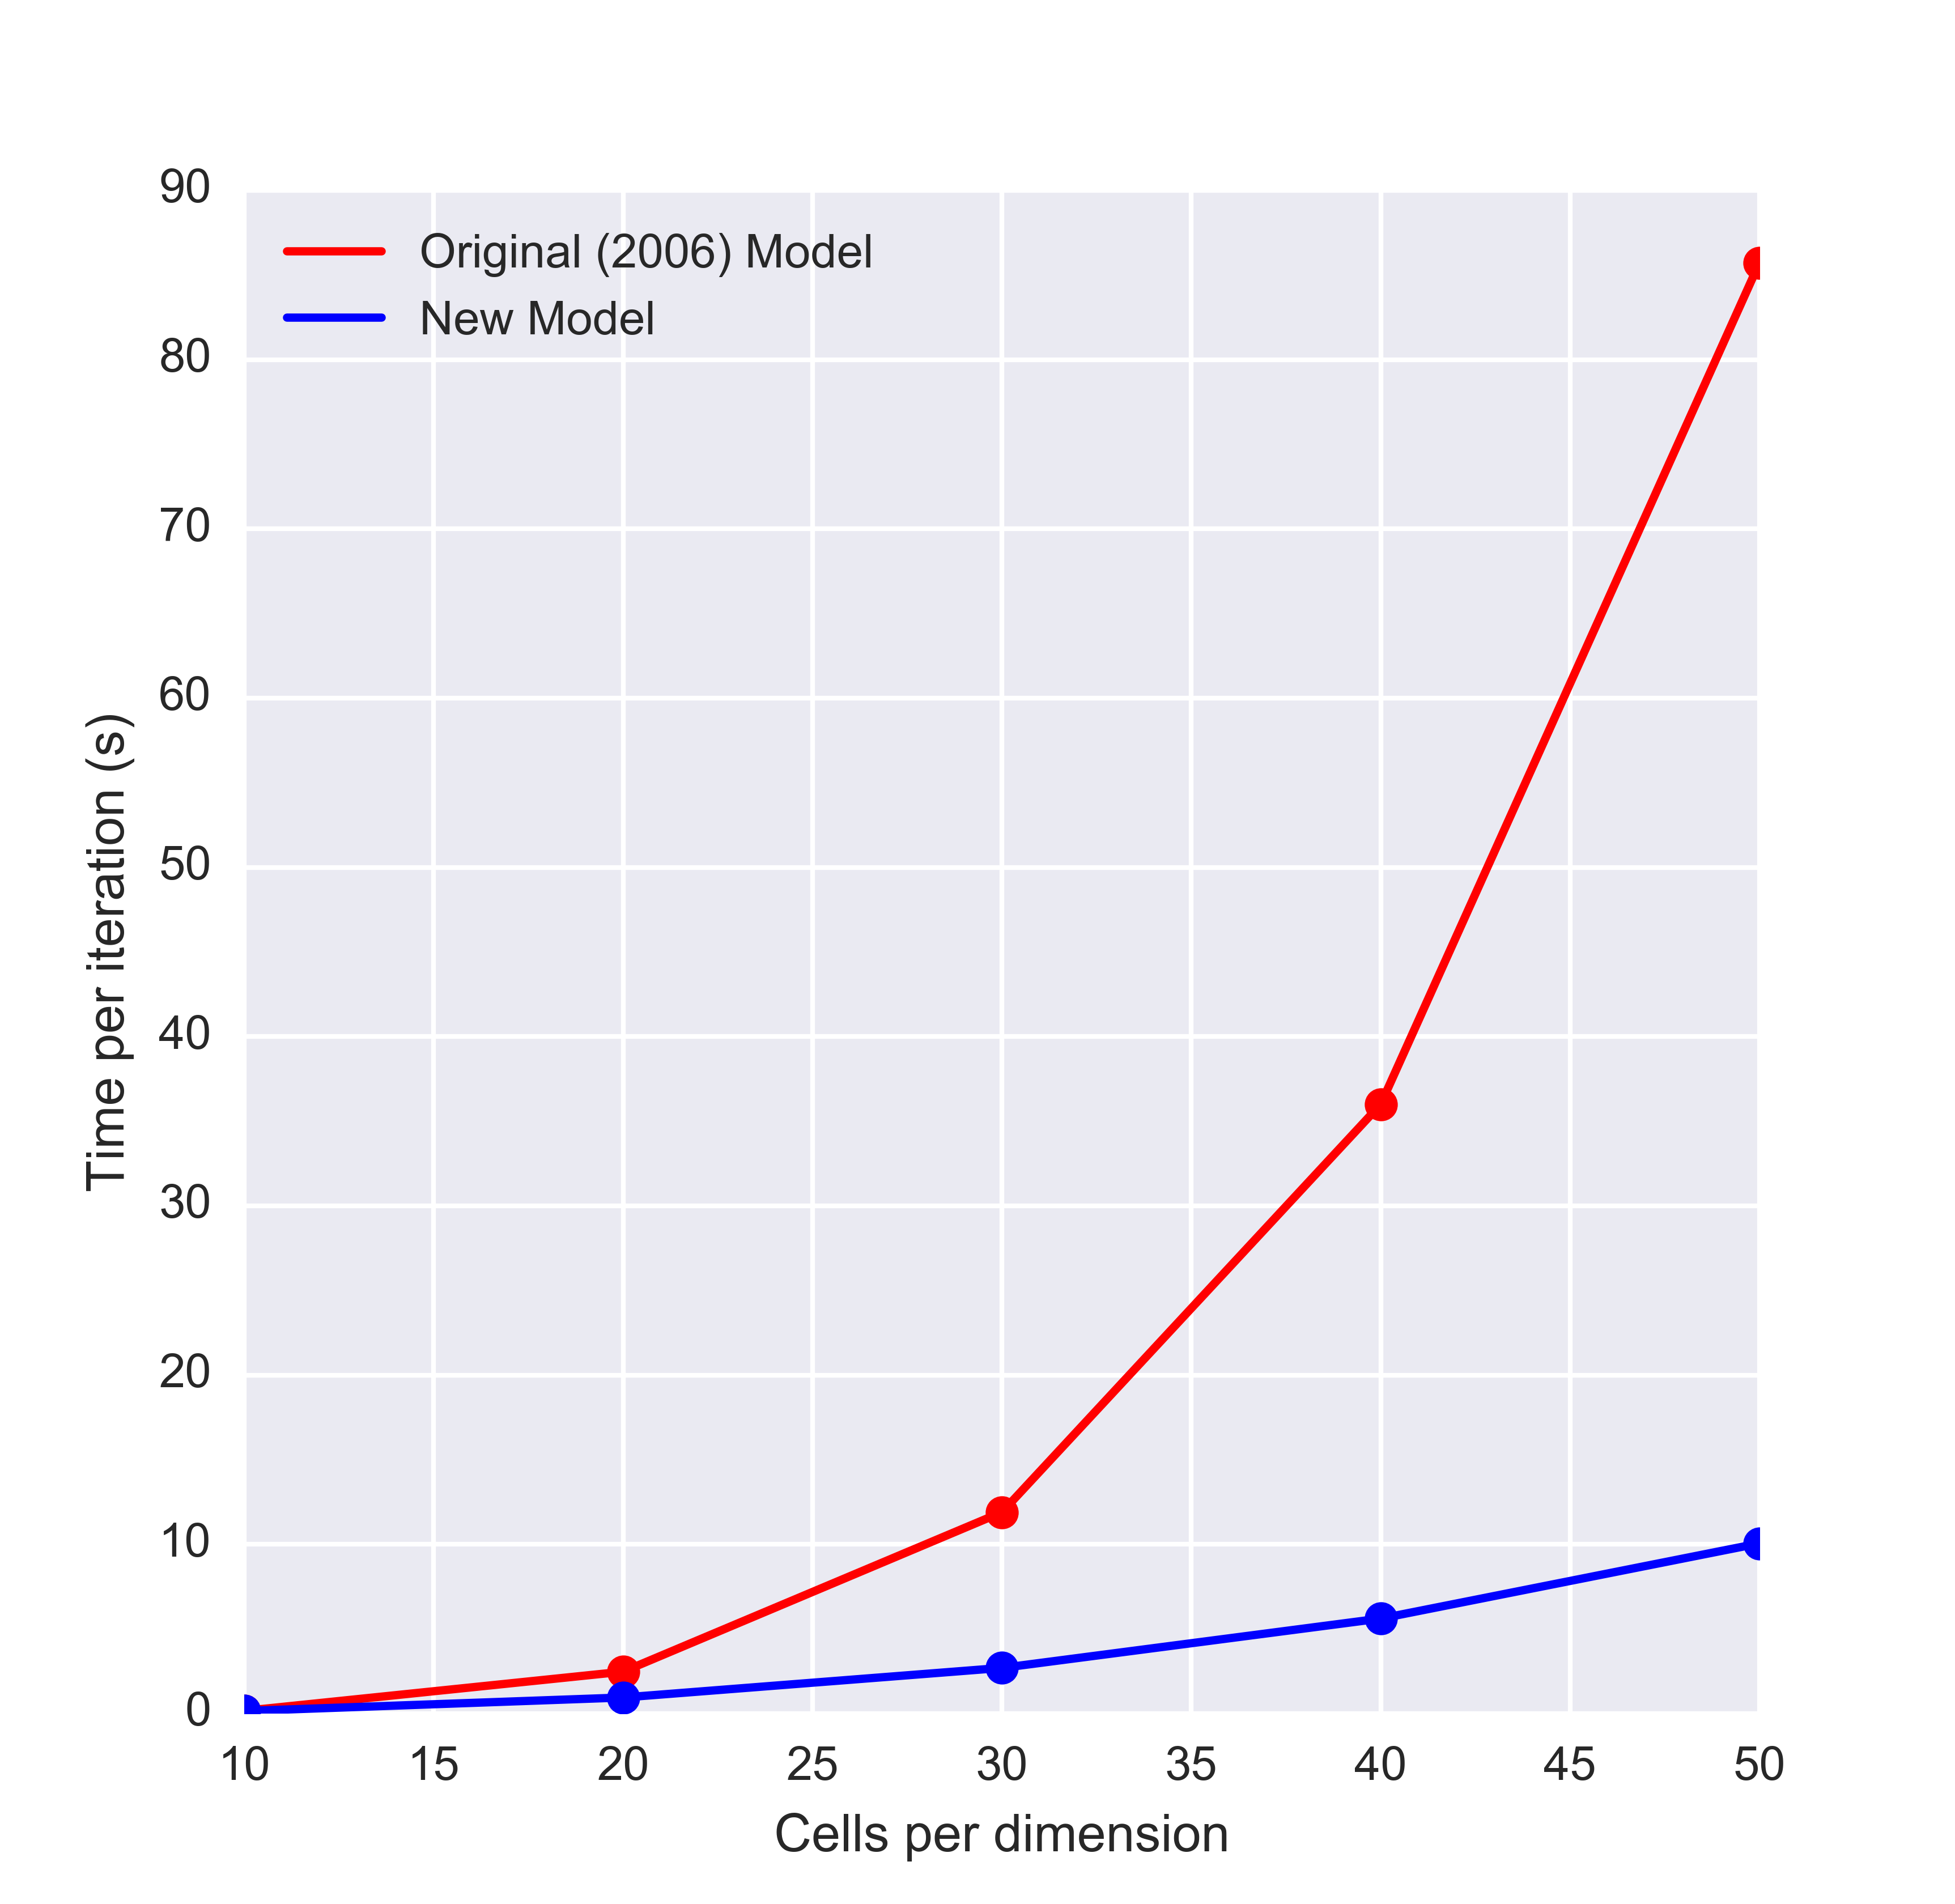
\includegraphics[scale=0.6]{ComputerSpeed}
\caption{\setstretch{1.0}\textbf{Model performance comparison.} Time per iteration to simulate systems of different sizes. Simulations were run with equal sized square retinas and tectums, so the horizontal axis represents the size of all four anatomical dimensions.}
\end{SCfigure}


\section{Discussion}

\textbf{Project outcomes}

{\setstretch{1.4}
Building a working model from the limited information available proved a difficult challenge. Myself coming from an experimental background with little prior modelling experience, this goes to highlight the current barrier that experimental biologists in the field must face in order to complement their experimental studies with computer modelling. I hope that in sharing my approach in an upcoming tutorial paper, as well as making publicly available the computer code that I generated, this barrier will be lowered, and future reassessment of the marker-induction model will be made easier. \\

With its consideration of both Eph/ephrin gradients and synapse addition/removal reactions, the model presented in this report is the most biologically accurate version of the marker-induction model to date. These changes also made a strong contribution to the computational performance of the model, allowing larger systems to be simulated. As well as building the actual model, an important outcome of the project was the development of three simple, intuitive precision measures, which allow for a quantitative comparison of maps between simulations. Analysis of these measures over time also provides information on the sequence of events in map formation, which suggests separate phases of topography generation and placement correction. As well as being a useful tool in the context of the marker-induction model, the three measures could also be applied to other similar models, and be a useful tool in model comparisons. A limitation of the measures is that we do know what values they actually take in real maps. Scores have been compared to the theoretical optimum values, but  real maps may not actually reach these precision levels. Current data on connectivity patterns in maps is not detailed enough to apply these measures. \\


I devoted the rest of the project to fully testing my model in a number of abnormal situations. I present for the first time a comprehensive analysis of surgery operations in a two-dimensional Eph/ephrin-dependent marker-induction model, demonstrating that the updated model retains its systems-matching properties. In addition, I show that the new version of the marker-induction model can recapitulate the results of \textit{EphA3}-knockin studies. Finally, by testing map generation with a range of tectal gradients, I demonstrate the importance of tectal information, and make predictions beyond what is currently experimentally available about the necessary strength of tectal gradients. \par
}

\pagebreak

In building the new version of the model it was necessary to change some of the parameters to improve its performance, most notably a weaker receptor-ligand comparison, and stronger tectal neighbour communication. Importantly I show that a model with a constant parameter set, optimised for normal simulations, can account for multiple experimental findings in abnormal simulations. Since these parameters do not have a clear quantifiable biological analogue, the biological significance of these changes is difficult to assess.
\\


\textbf{Remaining limitations of the marker-induction model}

The model is still highly abstract, and ignores many mechanistic details. An example of this is the synapse normalisation term, which is included without any consideration of cellular mechanisms. Also, a consequence of parameters having no real biological units is that the model has no consideration of absolute time, which prevents comparison with the timing of real development. The model is also currently limited to analysis of systems far smaller than reality. The retina has been predicted to contain around 50,000 RGCs (Salinas-Navarro et al., 2009), far more than the 2,500 used in my largest simulations. For many purposes this is likely already sufficient, as the systems tested here are already large enough that the system boundaries affect only a small part of the overall map. Scaling systems up beyond this would only be required to assess the effects of heterogeneities across the retina and tectum. RGC density, for example, is assumed to be constant in the model, but has been found to vary across the retina of mice (Jeon et al., 1998). Overall, despite its simplifications, the model in its current form is a good representation of our level of understanding, and should not be made more complex until this is improved. \\

Perhaps the greatest limitation, however, is that we still lack any solid experimental data demonstrating that tectal markers are adaptable. Despite the marker-induction model being around for decades, very few researchers have attempted to monitor whether tectal gradients can change during development. In the few basic studies that have been performed, findings are conflicting and inconclusive (Rodger et al., 2000; Bach et al., 2003). In order to fully test the accuracy of the marker-induction model, tectal ephrins should be monitored in scenarios where the model would predict a change, such as genetic manipulation of Eph gradients and mismatch surgery. Clearly, more evidence is needed, and without this evidence it will be impossible to assess the model's relevance. It is because of this that, despite its good ability to predict experimental data, the model remains highly controversial. \\

\textbf{Alternative models}

The marker-induction model is just one of many marker-dependent models proposed to account for map plasticity. Some alternative models propose that instead of individual RGCs having innate preferences for different tectal regions, all RGCs prefer the \textit{same} region of the tectum, but the strength of their affinity depends on their Eph levels. In these models, altered maps can be explained by altered levels of \textit{competition}, rather than altered gradients (Gierer, 1983; Whitelaw and Cowan, 1981).
\\

It is also important not to ignore the role of electrical activity. It is traditionally thought that activity-dependent and marker-dependent mechanisms act independently, with electrical activity serving mainly to refine maps once set up (Eglen and Gjorgjieva, 2009). Indeed, in stable maps generated from my marker only model, the mean RF diameter is larger than would be expected from a perfect 1:1 map, and systems-matching is close to, but not at the optimum level of 0, highlighting the need for further refinement. This ability of electrical activity to refine maps was computationally tested by Willshaw and von der Malsburg (1976) before their initial proposal of the marker-induction model. They showed that maps with an initial topographic bias in their connectivity patterns (now assumed to be set up by marker-dependent mechanisms), could be progressively refined by synchronised waves of neural activity. \\

Some studies, however, suggest that marker-based and electrical activity mechanisms may actually be functionally interlinked. Reports from Nicol et al. (2007) for example, suggest that the ability of ephrinA to act as a repellent cue can be modulated by electrical activity. Electrical activity is thought to influence marker-dependent map formation in the developing spinal cord (Hanson and Landmesser, 2004), and there may be mechanistic similarities here. Ideas can be tested using combined models of electrical activity and molecular markers. \\

\pagebreak

\textbf{Future work}

This report only presents model comparisons against a small amount of the experimental data available, and it would be interesting to see how well it fares against data from other studies (e.g. Eph and ephrin knockouts) with its current parameter set. Also, a priority in the short term should be attempting to further improve model performance. Despite the large improvements brought about by my changes to the model, I believe there are still improvements to be made in this regard. The high-performance programming languages Julia and Cython were touched upon in the project, but a lack of time prevented a full assessment of their power. Currently at roughly 10-15 hours running time per simulation, further speed improvements would go a long way to increasing the accessibility of the model, and may also permit implementation of proper parameter-optimisation protocols. \\

The main factor hindering progress in the field, however, is a lack of experimental data, and this should become the priority if we are to get any closer to understanding the mechanisms retinotopic map formation. Modelling and experimental approaches work best when used together, and currently the balance in the field is not complementary. In particular we need better quantitative information about retinal and tectal gradients in normal stable maps, in abnormal maps from genetic studies and surgical manipulations, and at different stages of development. Current data is poor, especially for tectal gradients and countergradients. We also lack detailed knowledge of the differences between species. The model in its current form is effectively species-less, and has been used unchanged in comparison with experimental data from different species, assuming identical mechanisms. Once new data is available, the progress made in this project should make it easier for researchers to test and build on the marker-induction model. This will then allow for a fuller test of the assumptions of the model, and permit increases to its complexity.


\section{Acknowledgements}

I would like to thank Stephen Eglen for all his work in making this project possible. His continued advice throughout the project was invaluable, and I thank him for taking the time to read through and give me feedback on the initial drafts of this report.


\section{Bibliography}

{\setstretch{1.0}
Abbott, L.F. (2008). Theoretical Neuroscience Rising. Neuron 60, 489–495. \\

Bach, H., Feldheim, D.A., Flanagan, J.G., and Scalia, F. (2003). Persistence of graded EphA/Ephrin-A expression in the adult frog visual system. J. Comp. Neurol. 467, 549–565. \\

Bednar, J.A., and Wilson, S.P. (2016). Cortical Maps. The Neuroscientist 22, 604–617. \\

Bekesy, G. von, and Wever, E.G. (1960). Experiments in hearing. (New York: McGraw-Hill). \\

Brown, A., Yates, P.A., Burrola, P., Ortuno, D., Vaidya, A., Jessell, T.M., Pfaff, S.L., O'Leary, D.D., and Lemke, G. (2000). Topographic mapping from the retina to the midbrain is controlled by relative but not absolute levels of EphA receptor signaling. Cell 102, 77–88. \\

Cheng, H.-J., Nakamoto, M., Bergemann, A.D., and Flanagan, J.G. (1995). Complementary gradients in expression and binding of ELF-1 and Mek4 in development of the topographic retinotectal projection map. Cell 82, 371–381. \\

Eglen, S.J., and Gjorgjieva, J. (2009). Self-organization in the developing nervous system: theoretical models. HFSP J. 3, 176–185. \\

Feldheim, D.A., Kim, Y.-I., Bergemann, A.D., Frisen, J., Barbacid, M., and Flanagan, J.G. (2000). Genetic Analysis of Ephrin-A2 and Ephrin-A5 Shows Their Requirement in Multiple Aspects of Retinocollicular Mapping. Neuron 25, 563–574. \\

Gaze, R.M., and Sharma, S.C. (1970). Axial differences in the reinnervation of the goldfish optic tectum by regenerating optic nerve fibres. Exp. Brain Res. 10, 171–181. \\

Gierer, A. (1983). Model for the Retino-Tectal Projection. Proc. R. Soc. Lond. B Biol. Sci. 218, 77–93. \\

Goodhill, G.J. (2007). Contributions of Theoretical Modeling to the Understanding of Neural Map Development. Neuron 56, 301–311. \\

Hanson, M.G., and Landmesser, L.T. (2004). Normal Patterns of Spontaneous Activity Are Required for Correct Motor Axon Guidance and the Expression of Specific Guidance Molecules. Neuron 43, 687–701. \\

Hebb, D. (1949). The Organisation of Behaviour (Wiley, New York). \\

Hjorth, J.J.J., Sterratt, D.C., Cutts, C.S., Willshaw, D.J., and Eglen, S.J. (2015). Quantitative assessment of computational models for retinotopic map formation. Dev. Neurobiol. 75, 641–666. \\

Horder, T.J. (1971). Retention, by fish optic nerve fibres regenerating to new terminal sites in the tectum, of “chemospecific” affinity for their original sites. J. Physiol. 216, 53P–55P. \\

Jeon, C.-J., Strettoi, E., and Masland, R.H. (1998). The Major Cell Populations of the Mouse Retina. J. Neurosci. 18, 8936–8946. \\

Kaas, J.H., and Catania, K.C. (2002). How do features of sensory representations develop? BioEssays 24, 334–343. \\

Malsburg, C.V.D., and Willshaw, D.J. (1977). How to Label Nerve Cells so that they can Interconnect in an Ordered Fashion. Proc. Natl. Acad. Sci. U. S. A. 74, 5176–5178. \\

Nicol, X., Voyatzis, S., Muzerelle, A., Narboux-Nême, N., Sudhof, T.C., Miles, R., and Gaspar, P. (2007). cAMP oscillations and retinal activity are permissive for ephrin signaling during the establishment of the retinotopic map. Nat. Neurosci. 10, 340–347. \\

O'Donovan, M.J. (1999). The origin of spontaneous activity in developing networks of the vertebrate nervous system. Curr. Opin. Neurobiol. 9, 94–104. \\

Reber, M., Burrola, P., and Lemke, G. (2004). A relative signalling model for the formation of a topographic neural map. Nature 431, 847–853. \\

Rodger, J., Bartlett, C.A., Beazley, L.D., and Dunlop, S.A. (2000). Transient Up-Regulation of the Rostrocaudal Gradient of Ephrin A2 in the Tectum Coincides with Reestablishment of Orderly Projections during Optic Nerve Regeneration in Goldfish. Exp. Neurol. 166, 196–200. \\

Salinas-Navarro, M., Jimenez-Lopez, M., Valiente-Soriano, F.J., Alarcon-Martinez, L., Aviles-Trigueros, M., Mayor, S., Holmes, T., Lund, R.D., Villegas-Perez, M.P., and Vidal-Sanz, M. (2009). Retinal ganglion cell population in adult albino and pigmented mice: A computerized analysis of the entire population and its spatial distribution. Vision Res. 49, 637–647. \\

Schmidt, J.., Cicerone, C.M., and Easter, S.. (1978). Expansion of the half-retinal projection to the tectum in goldfish: an electrophysiological and anatomical study. J Compo Neurol 177, 257–288. \\

Sperry, R.W. (1963). Chemoaffinity in the orderly growth of nerve fiber patterns and connections. Proc. Natl. Acad. Sci. U. S. A. 50, 703–710. \\

Whitelaw, V.A., and Cowan, J.D. (1981). Specificity and plasticity of retinotectal connections: a computational model. J. Neurosci. 1, 1369–1387. \\

Willshaw, D. (2006). Analysis of mouse EphA knockins and knockouts suggests that retinal axons programme target cells to form ordered retinotopic maps. Development 133, 2705–2717. \\

Willshaw, D.J., and von der Malsburg, C. (1976). How patterned neural connections can be set up by self-organization. Proc. R. Soc. Lond. B Biol. Sci. 194, 431–445. \\

Willshaw, D.J., and von der Malsburg, C. (1979). A marker induction mechanism for the establishment of ordered neural mappings: its application to the retinotectal problem. Philos. Trans. R. Soc. Lond. B. Biol. Sci. 287, 203–243.\par}


\end{document}